\documentclass[xcolor=table,hideothersubsections]{beamer}
\usepackage[utf8]{inputenc}

%\documentclass[xcolor=table,hideothersubsections,aspectratio=1610]{beamer}
%should do exactly that. Other possible values are: 1610, 169, 149, 54, 43 and 32.
%By default, it is to 128mm by 96mm(4:3).

\usefonttheme{structurebold}

\useoutertheme[height=36pt,width=1.86cm]{sidebar}
\usetheme{Berkeley}

%\usetheme[width=1.65cm]{Berkeley}

\beamertemplatenavigationsymbolsempty

\uselanguage{French}
\languagepath{French}
\useinnertheme{rounded}

\usepackage{color, colortbl}
\usepackage{tcolorbox}
\usepackage{multirow}
\usepackage{textcomp}
\usepackage{siunitx}
\usepackage{tikz}
\usepackage[safe]{tipa}
\usepackage{array}
\usepackage{hhline}
\usepackage{pbox}
\usepackage{etoolbox}
\usepackage{algorithm,algorithmic}

\usepackage{environ}

\tikzset{rndblock/.style={rounded corners,rectangle,draw,outer sep=0pt}}
\newcommand{\tframed}[2][]{\tikz[baseline=0.1pt]\vspace{0.1cm}\node[rndblock,minimum height=1.5em,#1] (m) {#2} ;}
\newcommand{\hilight}[1]{\textbf{\tframed[blue,fill=blue!10]{#1}}}
\newcommand{\whilight}[1]{\textbf{\tframed[purple,fill=purple!10]{#1}}}

% tkiz ball item
\newcommand*\circled[1]{\tikz[baseline=(char.base)]{\node[circle,ball color=darkcerulean, shade,
 color=white,inner sep=2.2pt] (char) {\tiny #1};}}

% tkiz rounded item
\newcommand*\rounded[1]{\tikz[baseline=(char.base)]{\node[draw=none,ball color=darkcerulean, shade,
 color=white, rounded corners=3.5pt, inner sep=2.5pt] (char) {\scriptsize #1};}}

%==============================================================================================================

\newcommand{\sP}{\hspace{1pt}}
\newcommand{\mP}{\hspace{3pt}}
\newcommand{\bP}{\hspace{6pt}}
\newcommand{\BP}{\hspace{12pt}}

\newcommand\fontJ{\fontfamily{ptm}\fontsize{6.1}{7.2}\selectfont}

\newcolumntype{L}[1]{>{\raggedleft\let\newline\\\arraybackslash\hspace{0pt}}m{#1}}
\newcolumntype{g}{>{\columncolor{tgray}}S[tabformat=2.2]}

%==============================================================================================================
\definecolor{darkcerulean}{rgb}{0.03, 0.27, 0.49}
\definecolor{bluepigment}{rgb}{0.2, 0.2, 0.6}
\definecolor{cobalt}{rgb}{0.0, 0.28, 0.67}
\definecolor{clearblue}{RGB}{135,206,250}
\definecolor{blendedblue}{rgb}{0.137,0.466,0.741}
\definecolor{defaultB}{rgb}{0.03, 0.27, 0.49}
\definecolor{darksalmon}{RGB}{233,150,122}
\definecolor{blendedgray}{rgb}{0.838,0.833,0.833}
\definecolor{blendedpurple}{RGB}{75,20,130}
\definecolor{tgray}{rgb}{0.211, 0.211,0.244}
\definecolor{darkgray}{rgb}{0.450,0.450,0.450}
\definecolor{maroon}{rgb}{0.665, 0.142, 0.142}
\definecolor{ngreen}{rgb}{0.000,0.500,0.000}


%==============================================================================================================
\newlength\leftsidebar
\newlength\rightsidebar
\makeatletter
\setlength\leftsidebar{\beamer@leftsidebar}
\setlength\rightsidebar{\beamer@rightsidebar}
\makeatother


%show current section and subsection
\makeatletter
\patchcmd{\insertverticalnavigation}%
{\ifx\beamer@nav@css\beamer@hidetext{\usebeamertemplate{section in sidebar}}\else{\usebeamertemplate{section in sidebar shaded}}\fi}%
{{\usebeamertemplate{section in sidebar}}}{}{}
\makeatother



% itemize
\setbeamercolor{item projected}{bg=darkcerulean}

\setbeamertemplate{itemize item}{\raise3.4pt\hbox{\donotcoloroutermaths\circled{}}}
\setbeamertemplate{itemize subitem}{\scriptsize\raise0.5pt\hbox{\donotcoloroutermaths\color{darkcerulean}$\ast$}} %\blacktriangleright
\setbeamertemplate{itemize subsubitem}{\scriptsize\raise0.5pt\hbox{\donotcoloroutermaths\color{darkcerulean}$\triangleright$}}
\setbeamertemplate{itemize/enumerate subbody begin}{\footnotesize}
\setbeamertemplate{itemize/enumerate subsubbody begin}{\scriptsize}

%\setbeamerfont{subsection in toc}{size=\small}

\setlength{\leftmargini}{10pt}
\setlength{\leftmarginii}{10pt}

%==============================================================================================================
\setbeamerfont{footline}{series=\bfseries}
\setbeamercolor{footline}{fg=darkcerulean}

\setbeamercolor{section in toc}{fg=darkcerulean}
\setbeamercolor{section number projected}{fg=white,bg=darkcerulean}

%\setbeamercolor{subsection in toc}{fg=darkcerulean}
%\setbeamercolor{subsection number projected}{fg=white,bg=darkcerulean}
%\setbeamercolor{subsection in toc shaded}{fg=darkcerulean!50}

\setbeamercolor{section in toc shaded}{fg=darkcerulean!50}
\setbeamercolor{section in sidebar shaded}{fg=darkcerulean!80}
\setbeamercolor{subsection in sidebar shaded}{fg=darkcerulean!80}

\setbeamercolor{sidebar}{fg=white,bg=darkcerulean}
\setbeamercolor{author in sidebar}{fg=clearblue}
\setbeamercolor{title in sidebar}{fg=clearblue}

\setbeamercolor{palette primary}{fg=white,bg=darkcerulean}
\setbeamercolor{palette secondary}{fg=white,bg=darkcerulean!108}
\setbeamercolor{palette structure}{fg=white,bg=darkcerulean}

\setbeamercolor{itemize item}{fg=darkcerulean,bg=darkcerulean}


%==============================================================================================================
\addtobeamertemplate{navigation symbols}{}{%
    \usebeamerfont{footline}%
    \usebeamercolor[fg]{footline}%
    \hspace{1em}%
    \insertframenumber/\inserttotalframenumber
}

\setbeamercolor{lowcol}{fg=black,bg=darkcerulean!30}

\newenvironment{titleblock}{
  \setbeamercolor{block title}{fg=white,bg=darkcerulean}
  \setbeamercolor{block body}{fg=white,bg=darkcerulean}
  \begin{beamerboxesrounded}[width=1.05\textwidth,shadow=true]
}{\end{beamerboxesrounded}}

\newenvironment<>{varblock}[2][\textwidth]{%
\vspace*{-20pt}
	  \setlength{\textwidth}{#1}
	  \begin{actionenv}#3%
	    \def\insertblocktitle{#2}%
	    \par%
	    \usebeamertemplate{block begin}}
	  {\par%
	    \usebeamertemplate{block end}%
	  \end{actionenv}
\vspace*{-20pt}
}

\newenvironment{variableblock}[3]{%
  \setbeamercolor{block body}{#2}
  \setbeamercolor{block title}{#3}
  \begin{block}{#1}
}{\end{block}}



%%%%%%%%%%%%%%%%%%%%%%%%%%%%%%%%%%%%%%%%%%%%%%%%%%%%%%%%%%%%%%%%%%%%%%%%%%%%%

\NewEnviron{specialannexe}[1][]{%
\begingroup
	\setbeamertemplate{footline}[frame number]{}
	\setbeamertemplate{navigation symbols}{}
	\setbeamertemplate{footline}{}

	\setbeamercolor{palette secondary}{fg=white,bg=darkcerulean}

	\makeatletter
	\setbeamertemplate{sidebar canvas left}{}
	\setbeamertemplate{sidebar left}{%
	  \vspace*{\fill}
	  \vspace*{\fill}
	}
	\makeatother

	\begin{frame}[noframenumbering,t]{\hskip-11ex Annexe}
	\makebox[\textwidth][c]{
	\begin{minipage}{\dimexpr\textwidth+0.25\textwidth\relax}
	\BODY
	\end{minipage}}
	\end{frame}
\endgroup
}

%%%%%%%%%%%%%%%%%%%%%%%%%%%%%%%%%%%%%%%%%%%%%%%%%%%%%%%%%%%%%%%%%%%%%%%%%%%%%

\newenvironment{specialframe}{%
    \begingroup
    \setbeamertemplate{navigation symbols}{}
    \begin{frame}[noframenumbering,plain]
}{\end{frame}
    \addtobeamertemplate{navigation symbols}{}{%
	\usebeamerfont{footline}%
	\usebeamercolor[fg]{footline}%
	\hspace{1em}%
	\insertframenumber/\inserttotalframenumber}
\endgroup}

\makeatletter
\long\def\beamer@@frametitle[#1]#2{%
  \beamer@ifempty{#2}{}{%
    \gdef\insertframetitle{\centering{#2\ifnum\beamer@autobreakcount>0\relax{}\space\usebeamertemplate*{frametitle continuation}\fi}}%
  \gdef\beamer@frametitle{#2}%
  \gdef\beamer@shortframetitle{#1}%
}%
}
\makeatother


%==============================================================================================================
% TOC
%==============================================================================================================

\AtBeginSection[]
{
	\hoffset=-.5\leftsidebar
	\begin{specialframe}
		\vskip-4ex
		\begin{variableblock}{}{bg=darkcerulean,fg=white}{}
		  \vskip1pt\hskip5pt\Large{\textbf{\color{white} Sommaire}}
		\end{variableblock}

		\vskip4ex

		\begin{minipage}{\textwidth}
			\linespread{1.4}
			\tableofcontents[currentsection, sectionstyle=show/shaded, hideothersubsections] %, subsectionstyle=hide/hide/hide, ]
		\end{minipage}


		%\tableofcontents[currentsection, hideothersubsections,sectionstyle=show/shaded, subsectionstyle=show/shaded/hide]
		%\vskip0.32mm
	\end{specialframe}
	\hoffset=0ex
}


%\AtBeginSubsection[]
%{
%	\hoffset=-.5\leftsidebar
%	\begin{specialframe}
%		\vskip4ex
%		\begin{variableblock}{}{bg=darkcerulean,fg=white}{}
%		  \vskip1pt\hskip5pt\Large{\textbf{\color{white} Sommaire}}
%		\end{variableblock}

%		\vskip4ex
%		\tableofcontents[currentsubsection, hideothersubsections,sectionstyle=show/shaded, subsectionstyle=show/shaded/hide]
%	\end{specialframe}
%	\hoffset=0ex
%}


%==============================================================================================================
% First slide
%==============================================================================================================
\title[RAPSODIE]{Reconnaissance de la parole \\pour l'aide à la communication \\pour les sourds et malentendants}
\author[Luiza Orosanu]{\textbf{\large Luiza Orosanu}\vskip-1cm}
\date{\footnotesize 11 décembre 2015}

\newcommand{\firstslide}
{
   \hoffset=-.5\leftsidebar
   \begin{specialframe}
	\begin{center}

	\vskip1ex
	\begin{titleblock}{}
	\centering\usebeamerfont{title}\inserttitle\par
	\end{titleblock}

	\vskip2ex
	\usebeamerfont{author}\insertauthor\par

	\vskip7ex
	\usebeamerfont{date}\insertdate\par

	\end{center}

	{\fontJ

	\vskip3ex\hskip5ex
	\textbf{\scriptsize Composition du jury}

	\vskip-3ex
	\begin{table}[h]
	\hspace*{8ex}\begin{tabular}{p{1.9cm}p{2.8cm}p{5.0cm}}
	\textit{Rapporteurs :}	& Laurent BESACIER 	& Prof., Universit\'{e} J. Fourier, LIG		\\
				& Georges LINAR\`{E}S 	& Prof., Universit\'{e} d'Avignon, LIA - CERI	\\
	\end{tabular}
	\end{table}

	\vskip-6ex
	\begin{table}
	\hspace*{8ex}\begin{tabular}{p{1.9cm}p{2.8cm}p{5.0cm}}
	\textit{Examinateurs :} & R\'{e}gine ANDR\'{E}-OBRECHT	& Prof., Universit\'{e} Paul Sabatier, IRIT 	\\
				& Martine ADDA-DECKER 		& DR CNRS, LPP					\\
				& Bernard GIRAU			& Prof., Universit\'{e} de Lorraine, Loria 	\\
	\end{tabular}
	\end{table}

	\vskip-6ex
	\begin{table}[h]
	\hspace*{8ex}\begin{tabular}{p{1.9cm}p{2.8cm}p{5.0cm}}
	\textit{Directeur de th\`{e}se :} & Denis JOUVET	& DR INRIA, Loria \\
	\end{tabular}
	\end{table}

	}

	\vskip-5ex
	\begin{table}[h]
	\hspace*{0.5ex}\begin{tabular}{ccccc}
	
\includegraphics{Image/logos/logo-LORIA.pdf} & 
\includegraphics[scale=0.2]{Image/logos/logo-INRIA.pdf} & 
\includegraphics[scale=0.6]{Image/logos/logo-UL.pdf}  & & 
\includegraphics[scale=0.09]{Image/logos/logo-CNRS.pdf}
	\end{tabular}
	\end{table}

   \end{specialframe}
   \hoffset=0ex
}


%==============================================================================================================
% document
%==============================================================================================================

\begin{document}

\firstslide


%==============================================================================================================
\section*{Contexte}
\begin{frame}[t]{Projet RAPSODIE}

\vspace{2ex}
\begin{columns}
	\begin{column}{.05\textwidth}
	\end{column}
	\begin{column}{.49\textwidth}
		\begin{center}
		{\bf \color{ngreen}R}econnaissance {\bf \color{ngreen}A}utomatique de la {\bf \color{ngreen}P}arole \\pour les personnes \\
		{\bf \color{ngreen}SO}urdes ou han{\bf \color{ngreen}DI}capé{\bf \color{ngreen}E}s
		\vspace{0.4cm}
		\end{center}
	\end{column}
	\begin{column}{.51\textwidth}
		
\includegraphics[scale=0.4]{Image/logos/logo-RAPSODIE}
	\end{column}
\end{columns}

\vskip5ex
{\bf \color{purple} \underline{Objectif}} : développer une nouvelle génération de \textbf{terminaux} proposant une reconnaissance vocale spécialisée sur les besoins des personnes sourdes ou malentendantes

\vskip3ex
{\color{darkcerulean}
{\fontencoding{U}\fontfamily{futs}\selectfont\char 66\relax} contexte initial embarqué}

\end{frame}


%==============================================================================================================
\begin{frame}[t]{Reconnaissance de la parole}

\vspace*{-2ex}
\begin{center}
\hspace*{-3ex}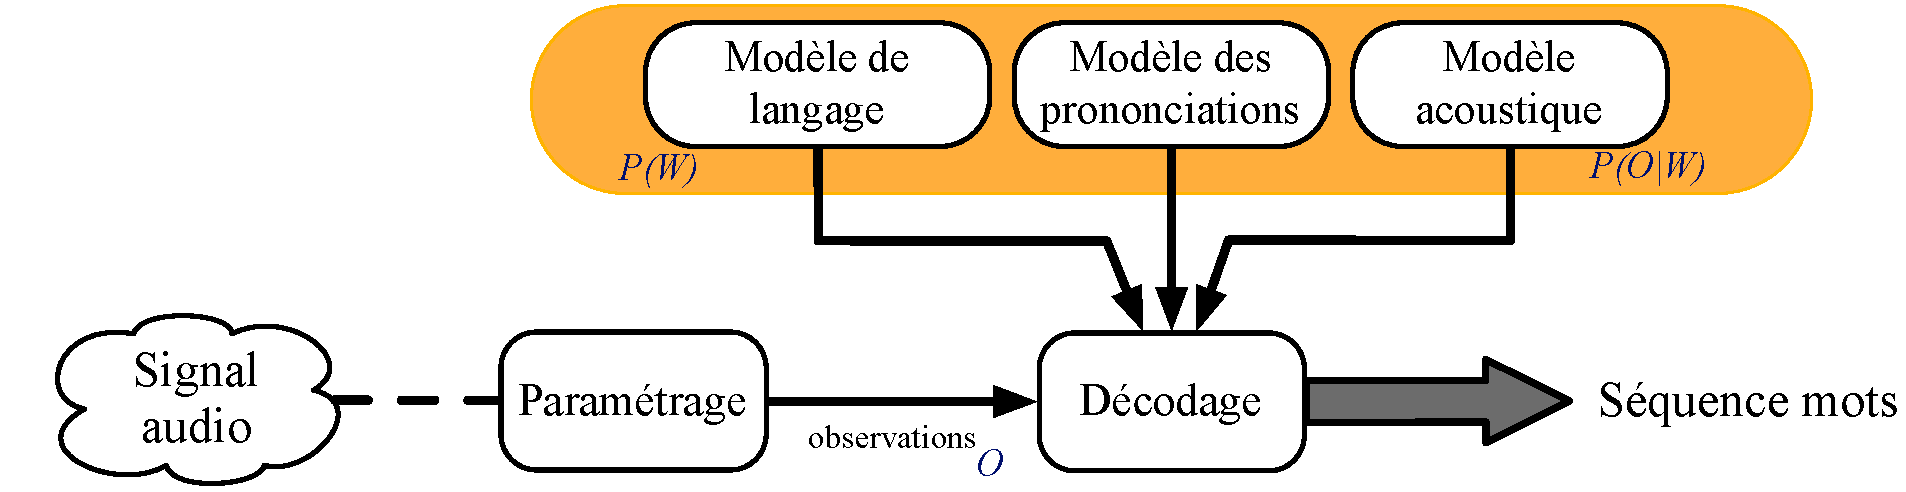
\includegraphics[scale=0.32]{Image/picture/rec_app_1.pdf}
\end{center}

\vskip1ex
{\footnotesize Étapes dans le processus de reconnaissance de la parole}

\begin{itemize}
\vspace*{2ex}
\item {\scriptsize analyse du signal}
\end{itemize}

\vskip2ex
\begin{columns}
	\begin{column}{.05\textwidth}
	\end{column}
	\begin{column}{.35\textwidth}
		\begin{itemize}
	   	\item \vskip-5ex{\scriptsize décodage utilisant}
	   	\end{itemize}
	\end{column}
	\begin{column}{.01\textwidth}
	\end{column}
	\begin{column}{.52\textwidth}
		\vskip-3ex\hskip-5ex$\left\{
                     \begin{array}{l}
			\text{\scriptsize modèle de langage}    	\\
	        	\text{\scriptsize modèle des prononciations}	\\
			\text{\scriptsize modèle acoustique}
                	\end{array}
                \right.$
	\end{column}
	\begin{column}{.2\textwidth}
	\end{column}
\end{columns}

\vskip3ex\hskip1ex{\color{purple}$\Rightarrow$} {\scriptsize la séquence de mots la plus vraisemblable}

\end{frame}


%==============================================================================================================
\begin{frame}[t]{\large Répondre aux besoins des personnes sourdes}

\only<1|handout:0>
{
	\vspace*{-3.2ex}
	\begin{center}
	\hspace*{-3.75ex}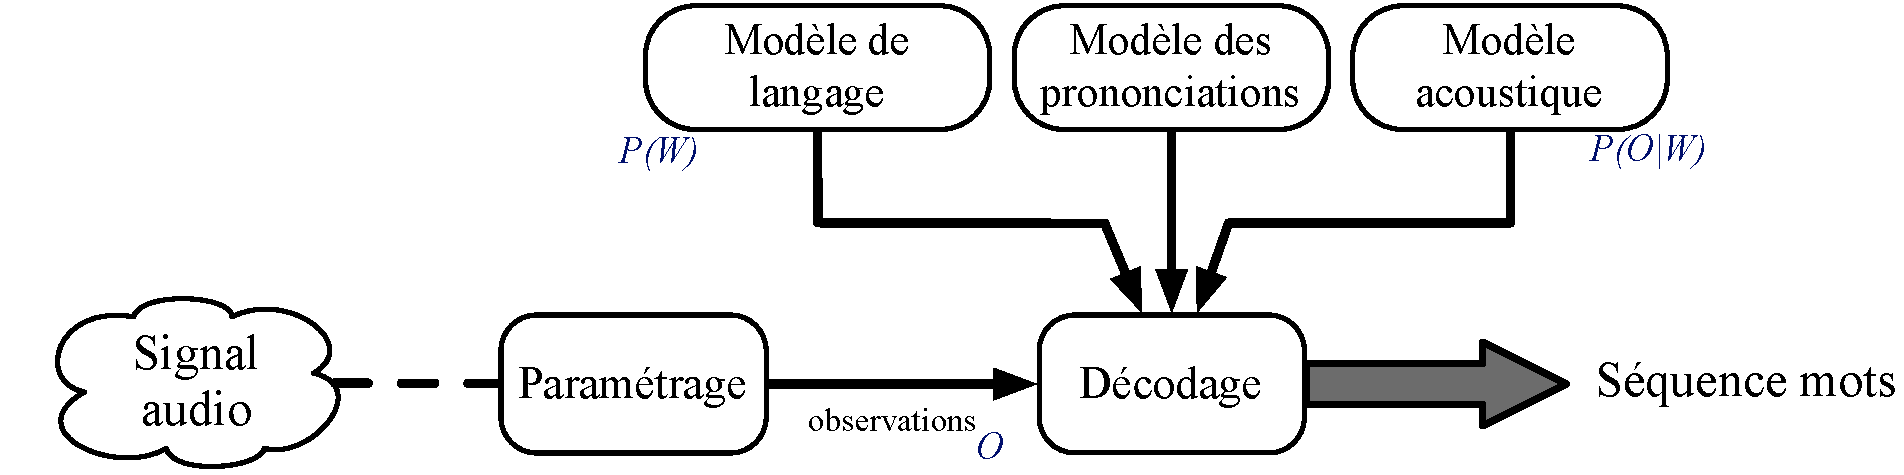
\includegraphics[scale=0.32]{Image/picture/rec_app_2-0.pdf}
	\end{center}

	\vspace{5ex}
}

\only<2|handout:0>
{
	\vspace*{-3.2ex}
	\begin{center}
	\hspace*{-3.75ex}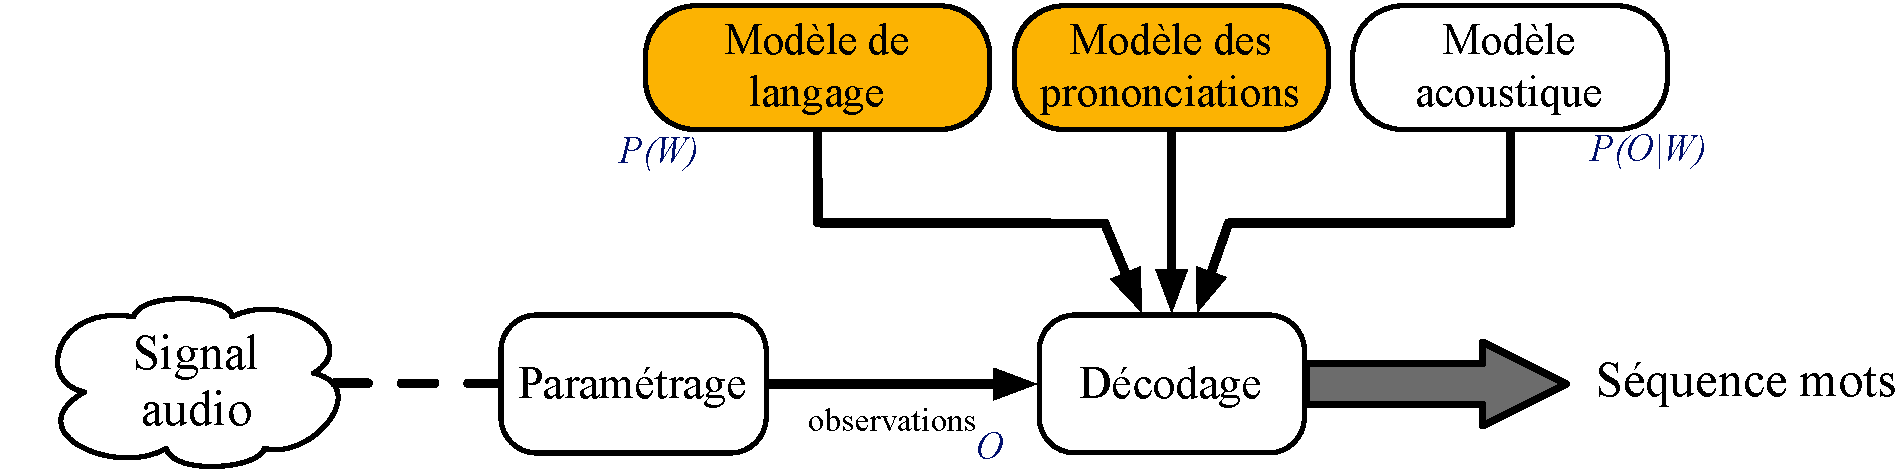
\includegraphics[scale=0.32]{Image/picture/rec_app_2.pdf}
	\end{center}

	\vspace{5ex}
}

\only<3->
{
	\vspace*{-6ex}
	\begin{center}
	\hspace*{-3ex}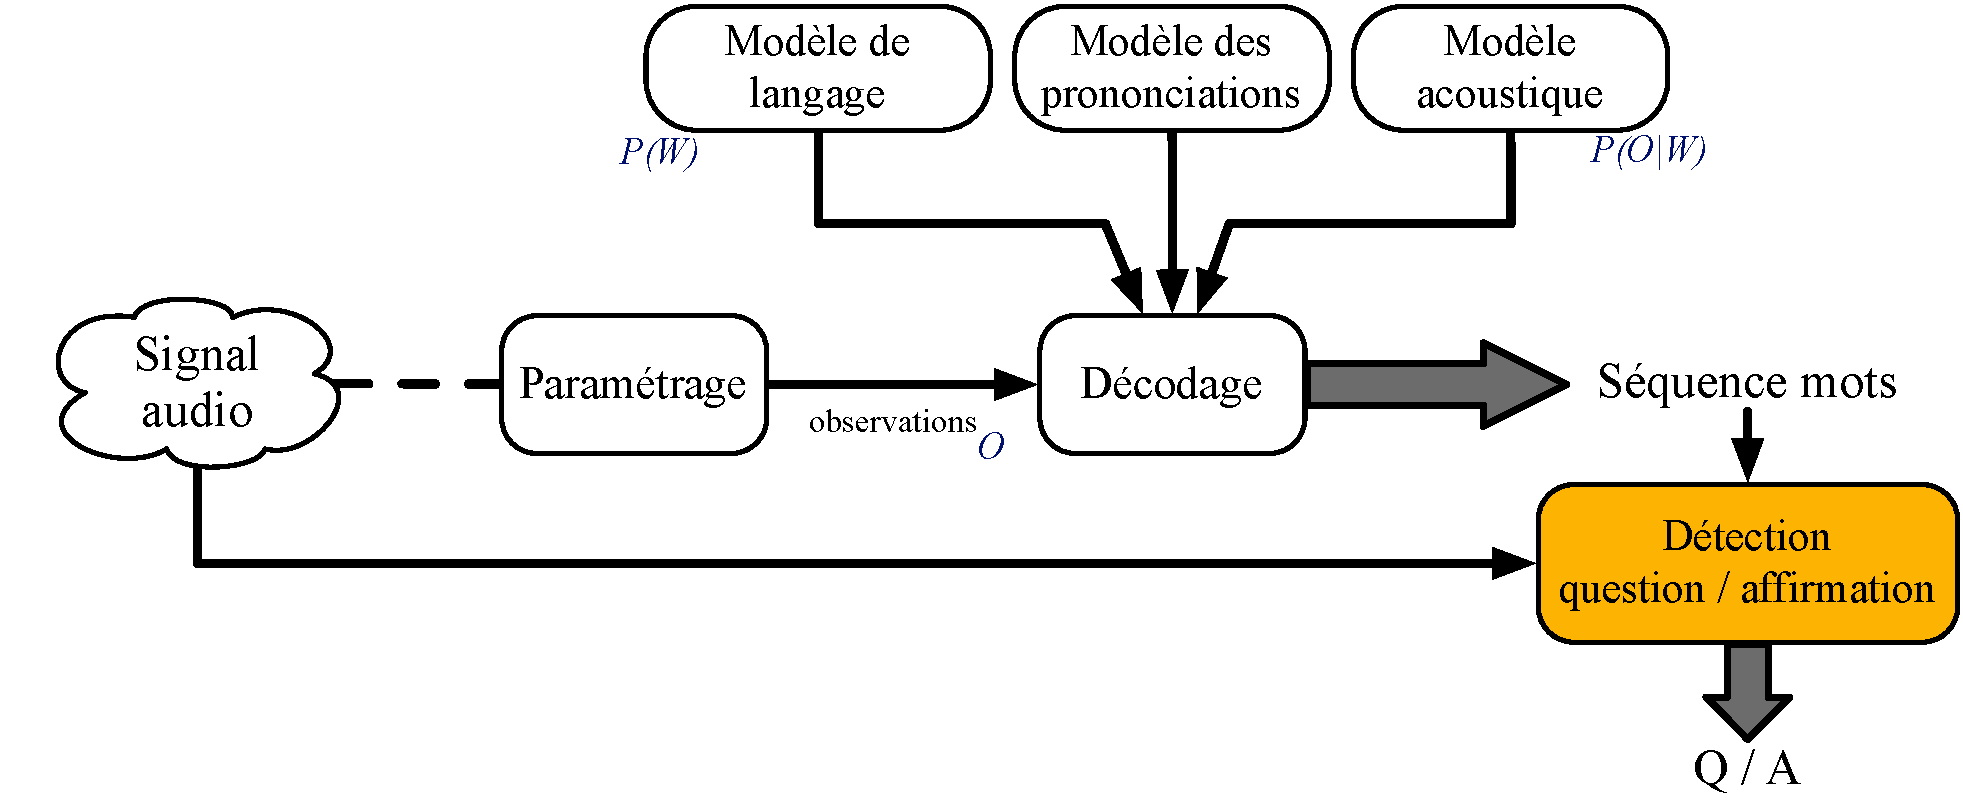
\includegraphics[scale=0.32]{Image/picture/rec_app_3_v2.pdf}
	\end{center}

	\vskip-5.3ex
}

\begin{itemize}
\item extraction d'\textbf{\color{purple} informations lexicales}

	\only<1|handout:0>
	{
		\vskip8.85ex
	}

	\only<2->
	{
		\begin{itemize}
		\vspace*{0.5ex}
		\item {\scriptsize choix d'unités pour le lexique et le modèle de langage $\Rightarrow$ {\color{blendedblue}modèles hybrides}}

		\vskip1ex
		\item  {\color{blendedblue}ajout de nouveaux mots} dans un modèle de langage
		\end{itemize}

		\vspace*{0.43ex}
	}

\item extraction d'\textbf{\color{purple}informations para-lexicales}

	\only<3->
	{
		\begin{itemize}
		\vspace*{0.5ex}
		\item détection automatique de {\color{blendedblue}questions et affirmations}
		\end{itemize}
	}
\end{itemize}

\end{frame}


%==============================================================================================================
\section{Modèles hybrides}
\subsection*{Problématique et approche}
\begin{frame}[t]{Modèles hybrides}

\begin{itemize}
\vskip4ex
\item \textbf{\color{purple}Problématique}

	\begin{itemize}
	\vskip2ex
	\item \textbf{\color{blendedblue}mots hors-vocabulaire} (quelle que soit la taille du vocabulaire)

		\vskip-0.3ex
		\hskip4ex\begin{beamerboxesrounded}[width=0.88\textwidth,shadow=true]{}
		\footnotesize
		\begin{center}
			\begin{tabular}{lcccccc}
			Référence : 	& dans & un & \multicolumn{2}{c}{village} 	& du & nord  \\
			Hypothèse : 	& dans & {\color{red}++parole++} & {\color{red}l'} & {\color{red}âge} & du & nord
			\end{tabular}
		\end{center}
		\end{beamerboxesrounded}

% dans(2) un village(2) kurde(2) du nord est
% dans(2) ++parole++ l' âge(2) du nord est

	\vskip2.5ex
	\item maximiser la \textbf{\color{blendedblue}compréhension de la transcription} résultante\\\vskip0.4ex pour la communauté de personnes sourdes

	\end{itemize}

\vskip4ex
\item \textbf{\color{purple}Modèle de langage hybride}
	\begin{itemize}
	\vskip2ex
	\item modèle combinant des mots avec des fragments de mots
	\end{itemize}

\end{itemize}

\end{frame}






%==============================================================================================================
\begin{frame}[t]{État de l'art des modèles hybrides}

{\footnotesize
\begin{itemize}
\vskip6ex
\item mots avec des phonèmes ou des syllabes \\{\color{gray}(anglais)} {\fontfamily{qcs}\selectfont \scriptsize \color{blendedblue} [Yazgan et Saraclar 2004]}

\vskip4ex
\item mots avec des graphones (ensemble lettres et phonèmes) \\ {\color{gray}(anglais)} {\fontfamily{qcs}\selectfont \scriptsize \color{blendedblue} [Bisani et Ney 2005]}

\vskip4ex
\item mots avec des séquences de phonèmes de longueurs variables \\ {\color{gray}(anglais)} {\fontfamily{qcs}\selectfont \scriptsize \color{blendedblue} [Rastrow et al. 2009]}

\vskip4ex
\item mots avec des morphèmes et des graphones à base de morphèmes  \\ ou mots avec des syllabes et des graphones à base de syllabes \\{\color{gray}(allemand)} {\fontfamily{qcs}\selectfont \scriptsize \color{blendedblue} [Shaik et al. 2011]}
\end{itemize}
}

\end{frame}



%==============================================================================================================
\begin{frame}[t]{Approche proposée}

\begin{itemize}
\vskip3ex
\item<1-> Choix d'un \textbf{\color{purple}modèle de langage hybride mots \& syllabes}
	\begin{itemize}
	\vskip1ex
	\item assurer une \textbf{\color{blendedblue}reconnaissance correcte des mots les plus fréquents}

	\vskip1ex
	\item proposer une suite de syllabes pour les mots hors-vocabulaire

     	\vskip2ex
	\hskip1ex\begin{beamerboxesrounded}[width=0.88\textwidth,shadow=false]{}
	\begin{center}
		{\color{purple}{\fontencoding{U}\fontfamily{futs}\selectfont\char 66\relax}}
	     		syllabes apprises à partir des \textbf{\color{blendedblue}prononciations réelles} \\
		\vskip0.7ex (1 syllabe $=$ 1 seule séquence de phonèmes $=$  1 prononciation)
	\end{center}
	\end{beamerboxesrounded}

	\end{itemize}

\vskip3ex
\item<2-> Motivations
	\begin{itemize}
	\vskip1ex
	\item \textbf{\color{purple} syllabes} {\color{darkcerulean}$\longleftarrow$} étude sur l'optimisation du décodage phonétique

	\vskip1ex
	\item \textbf{\color{purple} mots} \hskip2.7ex {\color{darkcerulean}$\longleftarrow$} entretiens effectués avec des personnes sourdes
	\end{itemize}
\end{itemize}

\only<3->
{
	\vskip1ex
	\hskip6ex\begin{beamerboxesrounded}[width=0.8\textwidth,shadow=true]{Exemple de transcription hybride}
	\footnotesize
	\begin{center}
		\begin{tabular}{ll}
		Reconnaissance : 	& une femme a été \ \_\textipa{b}\_\textipa{l}\_\textipa{e} \ \_\textipa{s}\_\textipa{e}  \\
		Affichage : 		& une femme a été \ \textipa{b} \textipa{l} \textipa{é} \textipa{s} \textipa{é}
		\end{tabular}
	\end{center}
	\end{beamerboxesrounded}
}

\end{frame}




%==============================================================================================================
\begin{frame}[t]{Corpus \& syllabation}

\begin{itemize}
\vskip1ex
\item<1-> Corpus d'apprentissage pour les modèles hybrides
	\begin{itemize}
	\vskip1.5ex
	\item {\footnotesize garder seulement les \textbf{\color{purple}mots les plus fréquents} {\color{gray}\scriptsize ($\#occ \ge N$)}}
	\vskip1.5ex
	\item {\footnotesize \textbf{\color{purple}décomposer en syllabes} les autres mots (peu fréquents)}
	\end{itemize}

\vskip2.5ex
\item<2-> Syllabation
	\begin{itemize}
	\vskip1.5ex
	\item alignement forcé \textbf{\color{purple}mots $\rightarrow$ phonèmes}

	\vskip1.5ex
	\item règles de syllabation \textbf{\color{purple}phonèmes $\rightarrow$ syllabes} \scriptsize{\color{blendedblue}[Bigi et al. 2010]}

	\only<3->
	{
		\begin{itemize}
		\vskip1ex
		\item {\scriptsize une syllabe contient une seule voyelle {\color{darkcerulean}(V)}}

		\vskip1ex
		\item {\scriptsize une pause désigne la frontière d'une syllabe}
		\end{itemize}

		\vskip3ex
		{\scriptsize
		\hspace*{0.5ex}\begin{tabular}{|c|c|c|lr|}
		\hline
		\textbf{Type de} & \textbf{Séquence de}	  	& \textbf{Position de}  & \multicolumn{2}{c|}{\textbf{Syllabes}}     \\
		\textbf{règle}   & \textbf{classes phonétiques} & \textbf{coupure} 	& \multicolumn{2}{c|}{\textbf{résultantes}}  \\ \hline
		GEN		 & {\color{darkcerulean}VV} 				& 0 	& {\color{darkcerulean}V}   & {\color{darkcerulean}V}	\\
		GEN		 & {\color{darkcerulean}V}x{\color{darkcerulean}V} 	& 0 	& {\color{darkcerulean}V}   & x{\color{darkcerulean}V}	\\
		GEN		 & {\color{darkcerulean}V}xx{\color{darkcerulean}V} 	& 1 	& {\color{darkcerulean}V}x  & x{\color{darkcerulean}V}	\\\hline
		EXC 		 & {\color{darkcerulean}V}OL{\color{darkcerulean}V}	& 0 	& {\color{darkcerulean}V}   & OL{\color{darkcerulean}V}	\\\hline
		\end{tabular}
		}
	}

	% diplomatie = d i p l oh m a s i = O V O L V O V O V = OV | OLV | OV | OV = d i | p l oh | m a | s i

	\end{itemize}
\end{itemize}

\end{frame}



%==============================================================================================================
\begin{frame}[t]{Exemple de syllabation}


\begin{center}
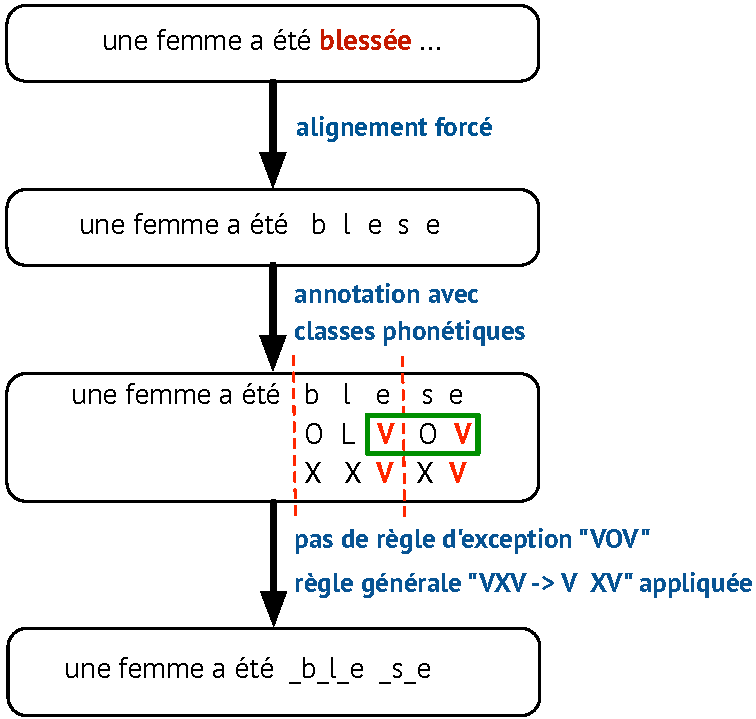
\includegraphics[scale=0.5]{Image/picture/syllabation-WS.pdf}
\end{center}

\end{frame}



%==============================================================================================================
\subsection*{Expérimentations}
\begin{frame}[t]{Fabrication des modèles hybrides}

\begin{itemize}

\vskip2ex
\item \textbf{\color{purple}Données textuelles des mots et syllabes}
   	\begin{itemize}
   	\vskip2ex
 	\item transcriptions manuelles des corpus de parole

 	\vskip2ex
 	\item critère de selection sur la fréquence d'occurrence des mots \\\vskip0.2ex\hskip3ex $\Rightarrow$ remplacement mots hors-vocabulaire par des syllabes
 	\end{itemize}

 	\vskip3ex
 	{\footnotesize Ensembles d'apprentissage d'\textbf{\color{blendedblue}ESTER2}, d'\textbf{\color{blendedblue}ETAPE} et d'\textbf{\color{blendedblue}EPAC} \\\vskip0.2ex\hskip3ex {\color{darkcerulean}$\rightarrow$}  {\scriptsize 3,6 millions de mots}}

	\vskip1ex
	{\scriptsize
	\begin{columns}
	\begin{column}{.25\textwidth}
	\flushright \textbf{\color{blendedblue} ESTER2 \& EPAC}
	\end{column}
	{\color{darkcerulean} \vrule height 0.3cm width 0.4pt}
	\begin{column}{.70\textwidth}
	   	\begin{list}{\color{darkcerulean}$\ast$}{\leftmargin=3mm \itemindent=0em}
			\item bulletins d'information français (radio)
			\item parole préparée, plus des interviews
		\end{list}
	\end{column}
	\end{columns}


	\vskip1ex
	\begin{columns}
	\begin{column}{.25\textwidth}
	\flushright \textbf{\color{blendedblue} ETAPE}
	\end{column}
	{\color{darkcerulean} \vrule height 0.3cm width 0.4pt}
	\begin{column}{.70\textwidth}
	   	\begin{list}{\color{darkcerulean}$\ast$}{\leftmargin=3mm \itemindent=0em}
			\item des débats (radio et télévision)
			\item parole spontanée
		\end{list}
	\end{column}
	\end{columns}
	}

\vskip4ex
\item \textbf{\color{purple}Outil d'apprentissage :} SRILM
\end{itemize}

\end{frame}




%==============================================================================================================
\begin{frame}[t]{Vocabulaires hybrides}

\begin{center}
\vskip-2ex
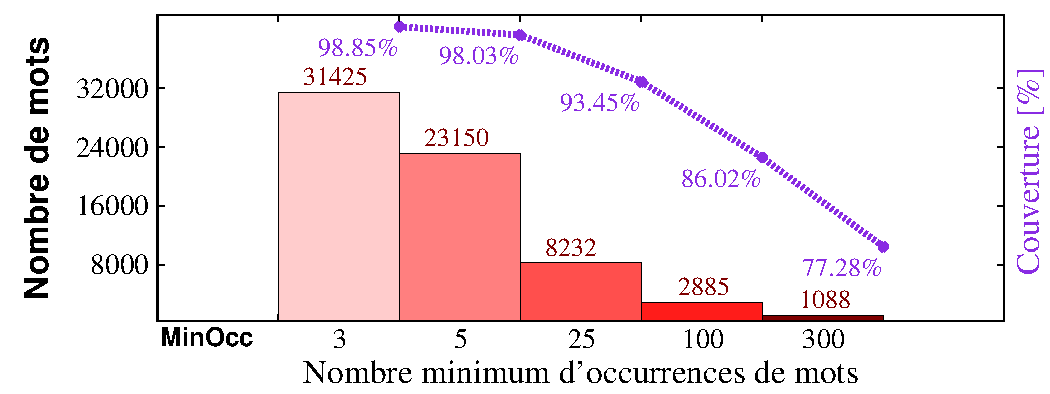
\includegraphics[scale=0.5]{Image/results/couverture_ws_minocc.pdf}
\vskip3ex
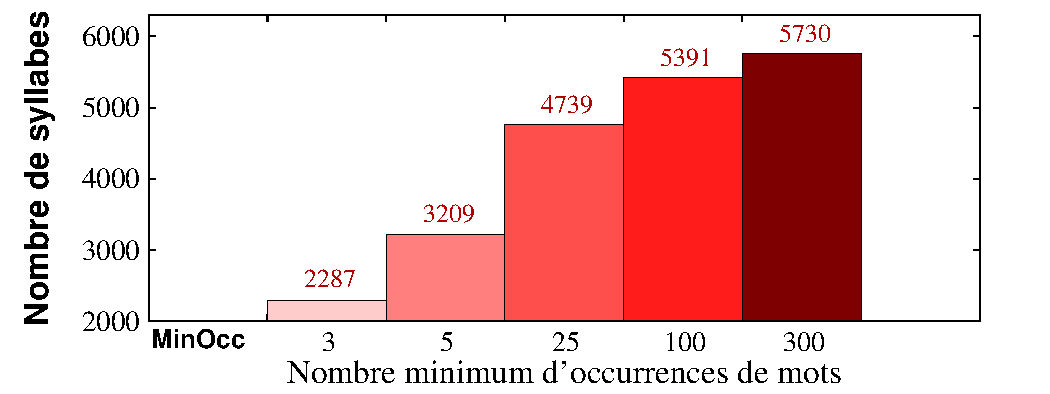
\includegraphics[scale=0.5]{Image/results/couverture_ws_s_minocc.pdf}
\end{center}

\end{frame}


%==============================================================================================================
\begin{frame}[t]{Évaluation}

\begin{itemize}

\vskip3ex
\item \textbf{\color{purple}Données d'évaluation}

	\begin{itemize}
	\vskip2ex
	\item ensemble de développement d'ESTER2 {\scriptsize\color{blendedblue}(parole préparée)}

	\vskip2ex
 	\item ensemble de développement d'ETAPE  {\scriptsize\color{blendedblue}(parole spontanée)}
 	\end{itemize}

\vskip3ex
\item Outils de décodage de la parole : \textbf{\color{purple}Sphinx3, PocketSphinx}

\end{itemize}

\only<2->
{
\vskip3ex
\hskip3ex\begin{beamerboxesrounded}[width=0.92\textwidth,shadow=true]{Modèles acoustiques}
	\footnotesize
	\begin{itemize}
		\item[$\ast$] \textbf{\color{purple}phonétiques HMM-GMM} dépendants du contexte
		\item[$\ast$] appris sur 300 heures de parole \\\vskip0.4ex $\rightarrow$ ensembles d'apprentissage d'ESTER2, d'ETAPE et d'EPAC
	\end{itemize}
	\end{beamerboxesrounded}
}

\end{frame}




%==============================================================================================================
\begin{frame}[t]{Évaluation des modèles hybrides}

\vskip2ex
\hskip6ex\begin{beamerboxesrounded}[width=0.8\textwidth,shadow=false]{}
	\footnotesize
	\begin{center}
		\begin{tabular}{ll}
		Modèle de mots : 	& une femme a été blessée \\
		Modèle hybride : 	& une femme a été \ \_b\_l\_e \ \_s\_e \\
		\end{tabular}
	\end{center}
	\end{beamerboxesrounded}

\only<2->
{
\begin{itemize}
\vskip4ex
\item \textbf{\color{purple}Performance des modèles hybrides}
	\begin{itemize}
	\vskip1.5ex
	\item<2-> taux d'erreur phonétique
	\vskip1.5ex
	\item<3-> taux de mots dans la transcription automatique
	\vskip1.5ex
	\item<4-> taux de mots et de syllabes correctement reconnus
	\vskip1.5ex
	\item<5-> taux de mots hors-vocabulaire reconnus par des syllabes
	\end{itemize}

\vskip4ex
\item<6-> Analyse des \textbf{\color{purple}mesure de confiance sur les mots}
	\begin{itemize}
	\vskip1.5ex
	\item[$\rightarrow$] décomposer en phonèmes les mots ayant une faible MC
	\end{itemize}

\end{itemize}
}

\end{frame}

%==============================================================================================================
\begin{frame}[t]{Taux d'erreur phonétique}

\only<1>
{
	\vspace*{-0.5ex}
	\begin{center}
	\hspace*{-1ex} 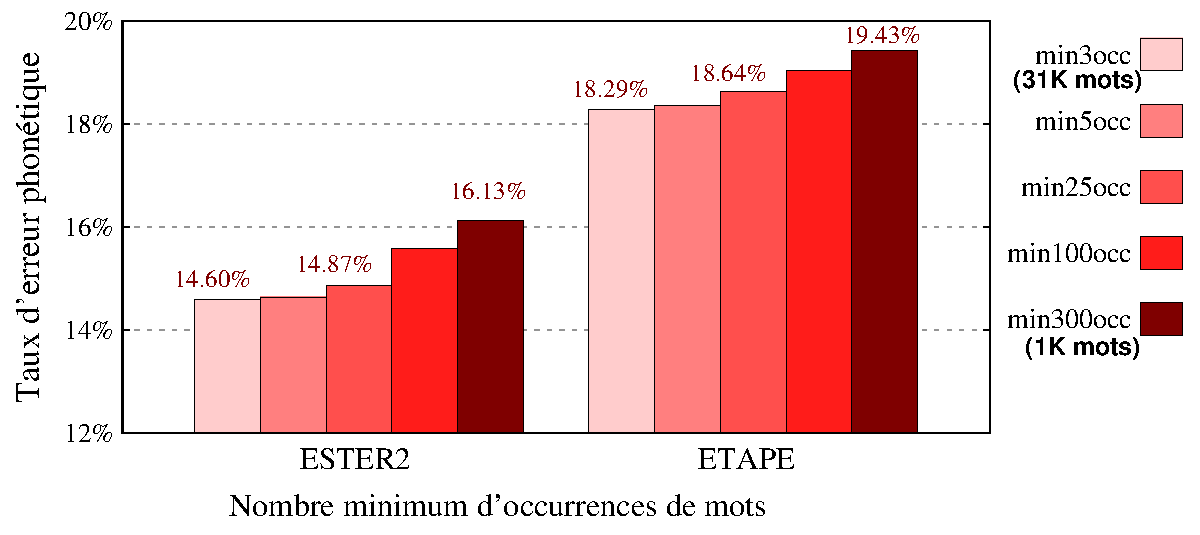
\includegraphics[scale=0.49]{Image/results/results_ws_minocc.pdf}
	\end{center}

	\vspace*{1.15ex}
	{\scriptsize
	\hskip1.32ex {\color{darkcerulean}$\Rightarrow$} \textbf{\color{purple}'min3occ'} (31K mots) : 14,60\% PER sur ESTER2, 18,29\% sur ETAPE}
}

\only<2|handout:0>
{
	\vspace*{-0.5ex}
	\begin{center}
	\hspace*{-1ex} 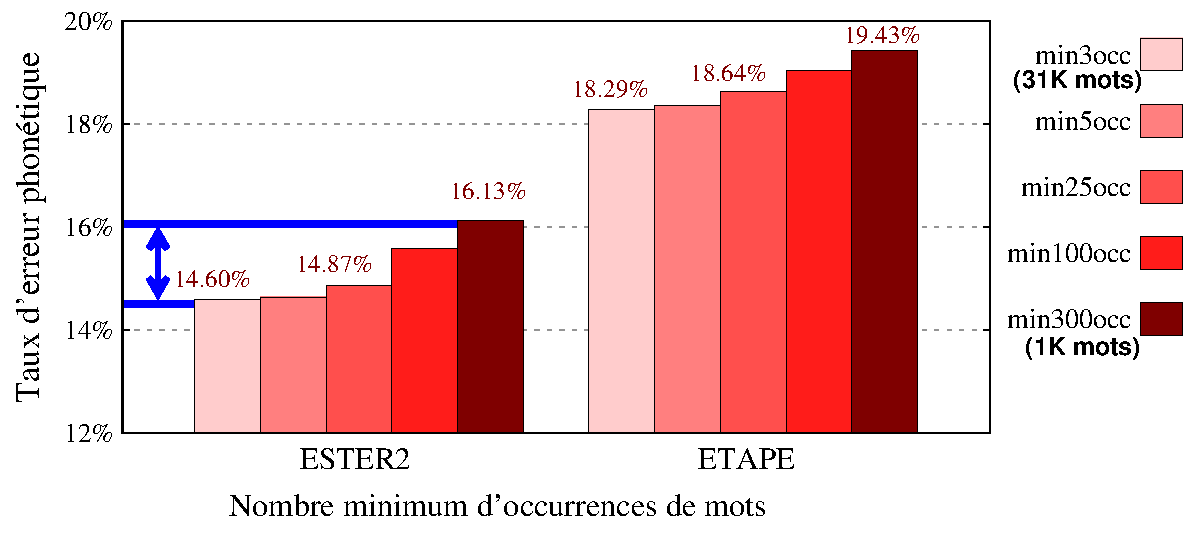
\includegraphics[scale=0.49]{Image/results/results_ws_minocc_c1.pdf}
	\end{center}


	\vspace*{0.5ex}
	\begin{columns}
	\begin{column}{0.5\textwidth}
	{\scriptsize {\color{darkcerulean}$\Rightarrow$} différence de performance de 1,5\%}
	\end{column}
	\begin{column}{0.4\textwidth}
	\hspace*{-4.5ex}$\left\{
                     \begin{array}{ll}
			\text{\scriptsize le plus grand vocabulaire (31K mots)}    	\\
			\text{\scriptsize le plus petit vocabulaire (1K mots)}
                	\end{array}
                \right.$
	\end{column}
	\end{columns}
}

\only<3-|handout:0>
{
	\vspace*{-0.5ex}
	\begin{center}
	\hspace*{-1ex} 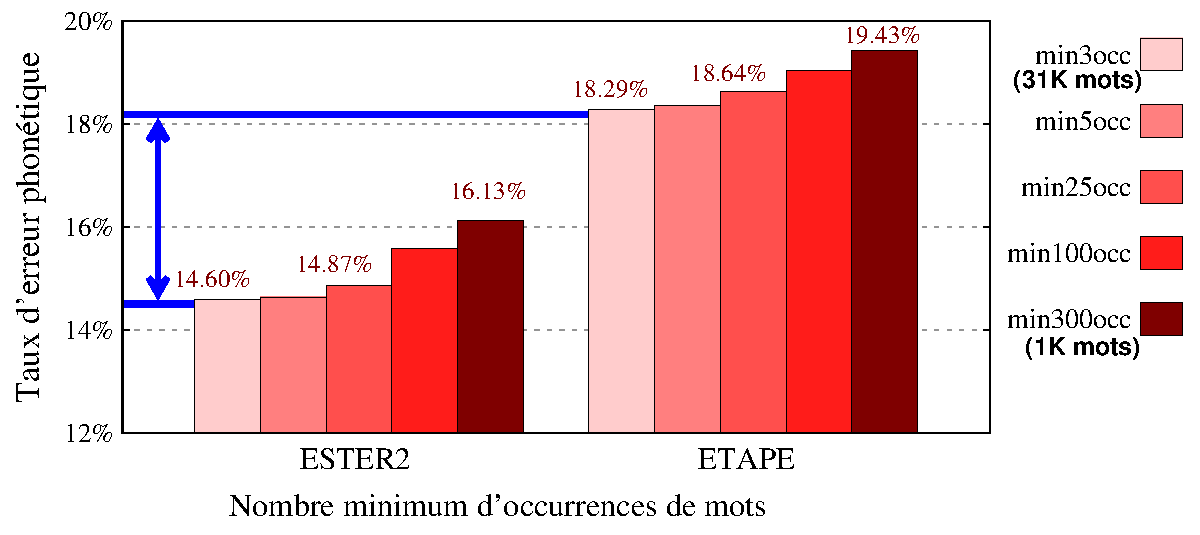
\includegraphics[scale=0.49]{Image/results/results_ws_minocc_c2.pdf}
	\end{center}

	\vspace*{0.5ex}
	\begin{columns}
	\begin{column}{0.5\textwidth}
	{\scriptsize {\color{darkcerulean}$\Rightarrow$} différence de performance de 3,7\%}
	\end{column}
	\begin{column}{0.4\textwidth}
	\hspace*{-4.5ex}$\left\{
                     \begin{array}{ll}
			\text{\scriptsize contexte de parole préparée}    	\\
			\text{\scriptsize contexte de parole spontanée}
                	\end{array}
                \right.$
	\end{column}
	\end{columns}
}

\end{frame}


%==============================================================================================================
\begin{frame}[t]{Taux de mots produits par le décodeur}

\begin{center}
\vskip-1.5ex
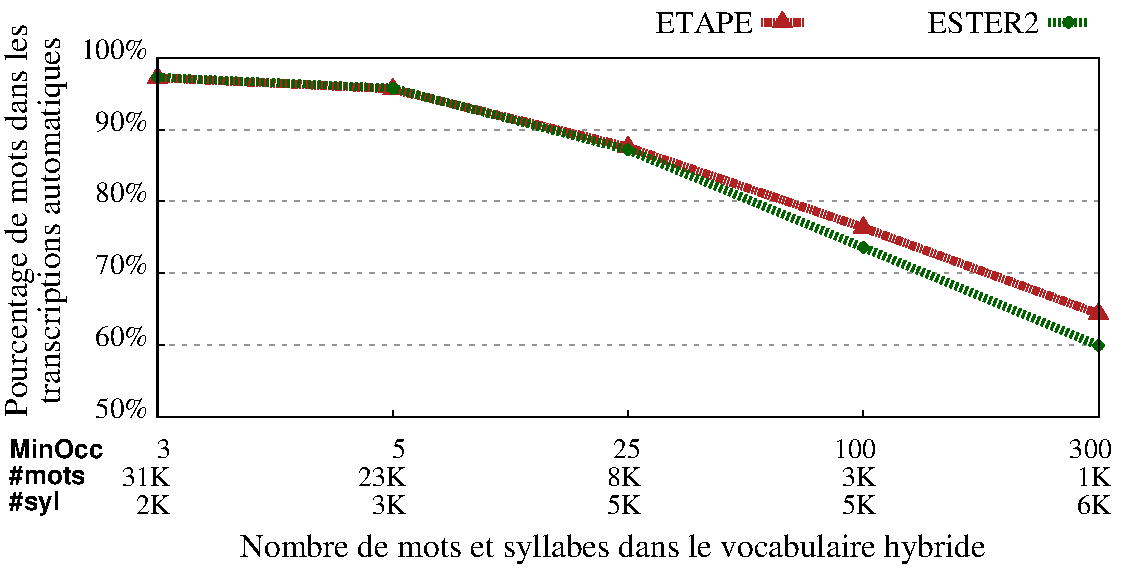
\includegraphics[scale=0.45]{Image/results/wordsInWS_sv.pdf}
\end{center}

\vskip-0.25ex
{\footnotesize
{\color{darkcerulean}$\Rightarrow$} les sorties de reconnaissance contiennent essentiellement des mots
}

\end{frame}



%==============================================================================================================
\begin{frame}[t]{Mots et syllabes correctement reconnus}

\only<1->
{
	\vspace*{-5ex}
	\begin{columns}
	\begin{column}{0.68\textwidth}
		\begin{center}
		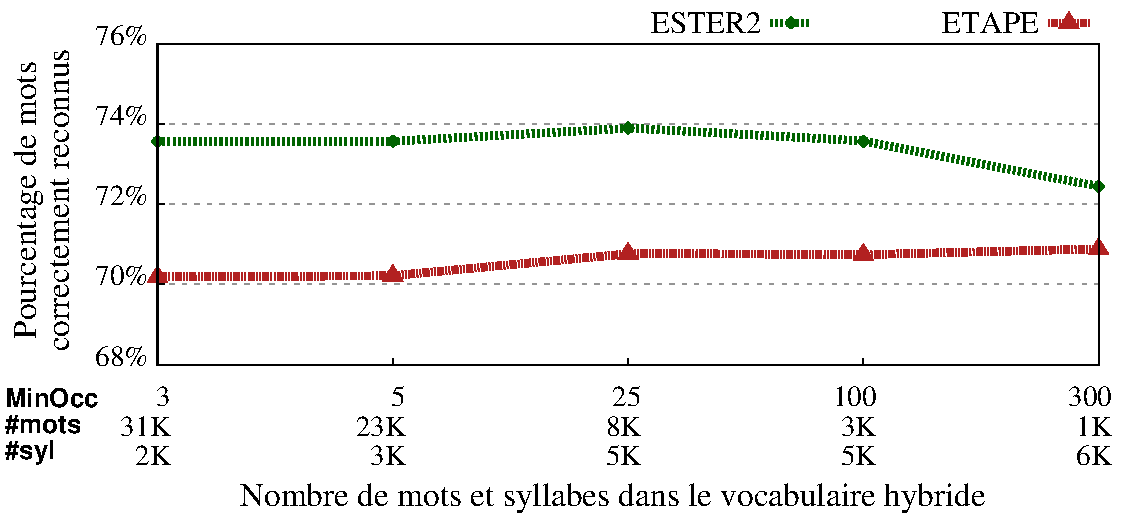
\includegraphics[scale=0.37]{Image/results/correctWordsInWS_sv.pdf}
		\end{center}
	\end{column}
	\begin{column}{0.37\textwidth}
		{\scriptsize
			\\\hskip0.5ex {\color{darkcerulean}$\Rightarrow$} \textbf{\color{blendedblue}mots corrects \\\hskip3.5ex parmi mots reconnus}
			\\\vskip1.5ex\hskip3.5ex {\color{darkcerulean}$\ast$} 73\% sur ESTER2
			\\\hskip3.5ex {\color{darkcerulean}$\ast$} 71\% sur ETAPE
		}
	\end{column}
	\end{columns}

}

\only<2->
{
	\vskip-3ex
	\begin{columns}
	\begin{column}{0.68\textwidth}
		\begin{center}
		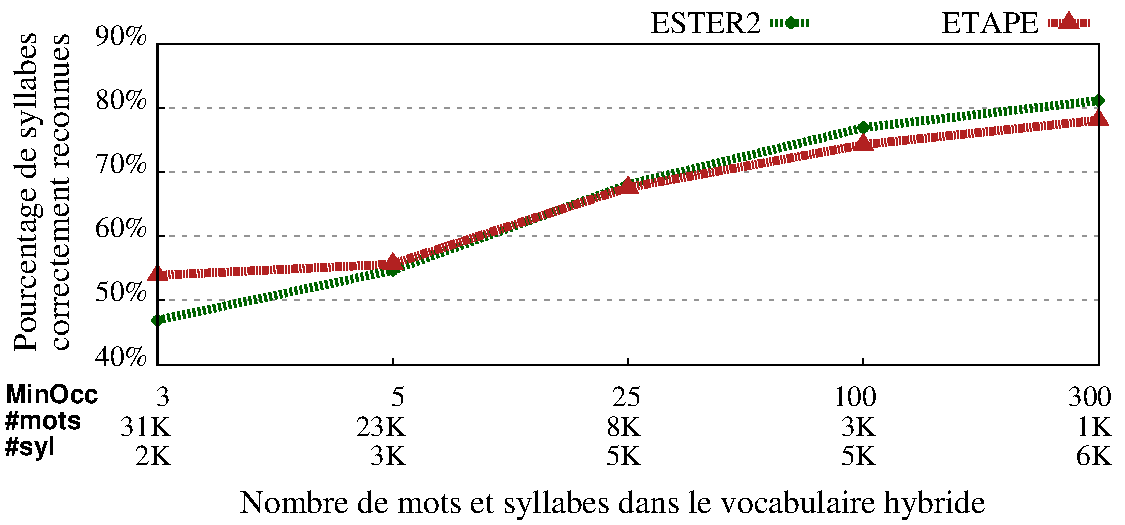
\includegraphics[scale=0.37]{Image/results/correctSyllablesInWS_sv.pdf}
		\end{center}
	\end{column}
	\begin{column}{0.37\textwidth}
		{\scriptsize
			\\\hskip0.5ex {\color{darkcerulean}$\Rightarrow$} \textbf{\color{blendedblue}syllabes correctes \\\hskip3.5ex parmi syllabes reconnues}
			\\\vskip1.5ex\hskip3.5ex {\color{darkcerulean}$\ast$} 46\% - 81\% sur ESTER2
			\\\hskip3.5ex {\color{darkcerulean}$\ast$} 54\% - 78\% sur ETAPE
		}
	\end{column}
	\end{columns}
}

\end{frame}


%==============================================================================================================
\begin{frame}[t]{Décodage des mots hors-vocabulaire}


\only<1->
{
	\vskip-1ex
	{\footnotesize L'ensemble de développement du corpus ESTER2} : {\scriptsize 41K occ. de mots}

	\vskip1ex
	{\scriptsize
	\hspace*{-4ex}
	\renewcommand{\arraystretch}{1.3}
	\begin{tabular}{|r|r|r|r|r|r|}
	\cline{2-6}
	\multicolumn{1}{c|}{}	  & min\textbf{3}occ	& min\textbf{5}occ & min\textbf{25}occ & min\textbf{100}occ & min\textbf{300}occ \\\hline
	\textbf{\% occ mots HV}  &  4,34 \%	& 5,11 \%	& 9,51 \%	& 16,98	\%	& 26,04	\%	\\\hline
	\end{tabular}
	}
}

\only<1|handout:0>
{
	\vskip5ex \hskip15ex 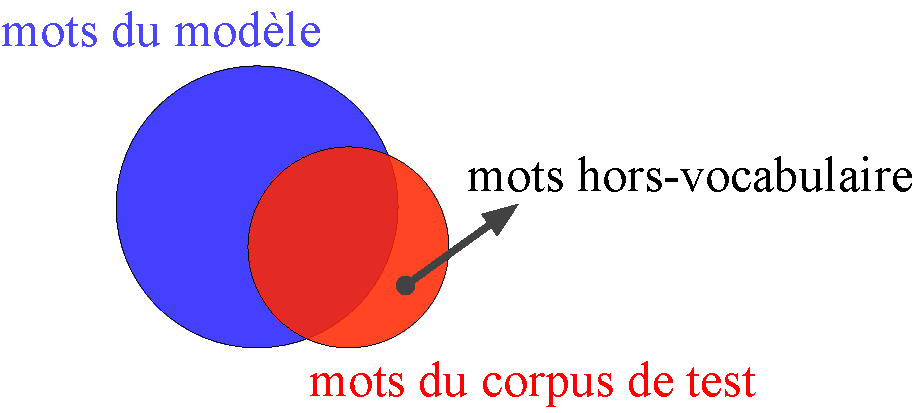
\includegraphics[scale=0.4]{Image/picture/vocabulary-fr.pdf}

}

\only<2->
{
	\begin{center}
	\vskip-3ex
	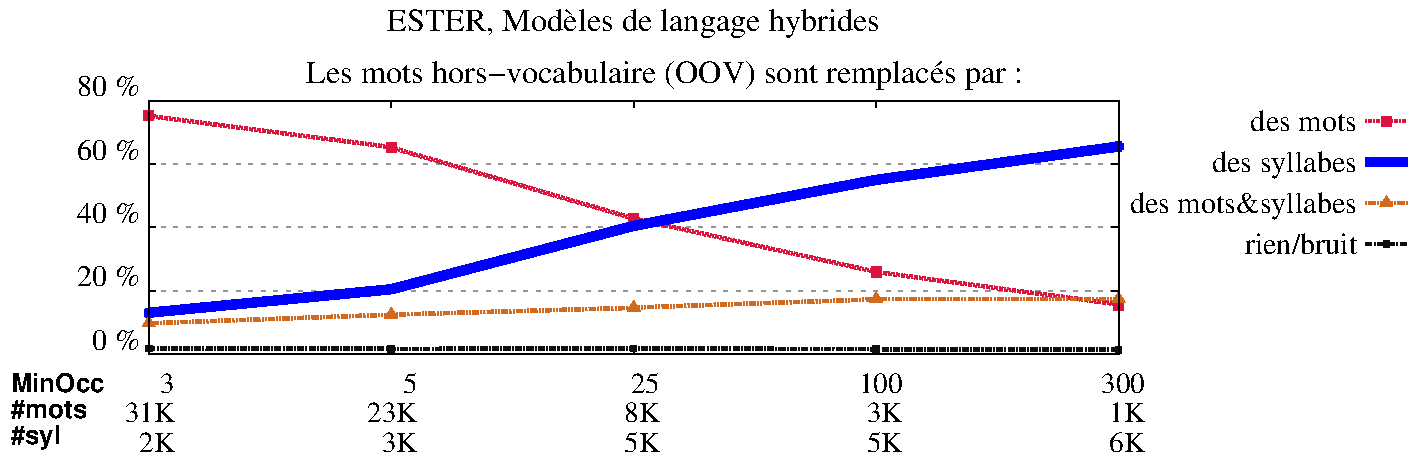
\includegraphics[scale=0.43]{Image/results/ESTER_OOV_sv.pdf}
	\end{center}

	\vskip0.1ex
	{\scriptsize
	{\color{darkcerulean}$\Rightarrow$} `min3occ' : {\scriptsize 75\% de mots hors-vocabulaire sont remplacés par d'autres mots}

	\vskip-0.1ex
	{\color{darkcerulean}$\Rightarrow$} `min300occ' : {\scriptsize 66\% de mots hors-vocabulaire sont remplacés par des syllabes}
	}
}

\end{frame}


%==============================================================================================================
\begin{frame}[t]{Mesures de confiance sur les mots}

\vspace*{-3ex}
\begin{columns}
\begin{column}{0.05\textwidth}
\end{column}
\begin{column}{0.2\textwidth}
\begin{center}
{\footnotesize Modèle évalué \\''min3occ``}
\end{center}
\end{column}
\begin{column}{0.6\textwidth}

\only<1|handout:0>
{
	\begin{center}
	\vskip-0.5ex
	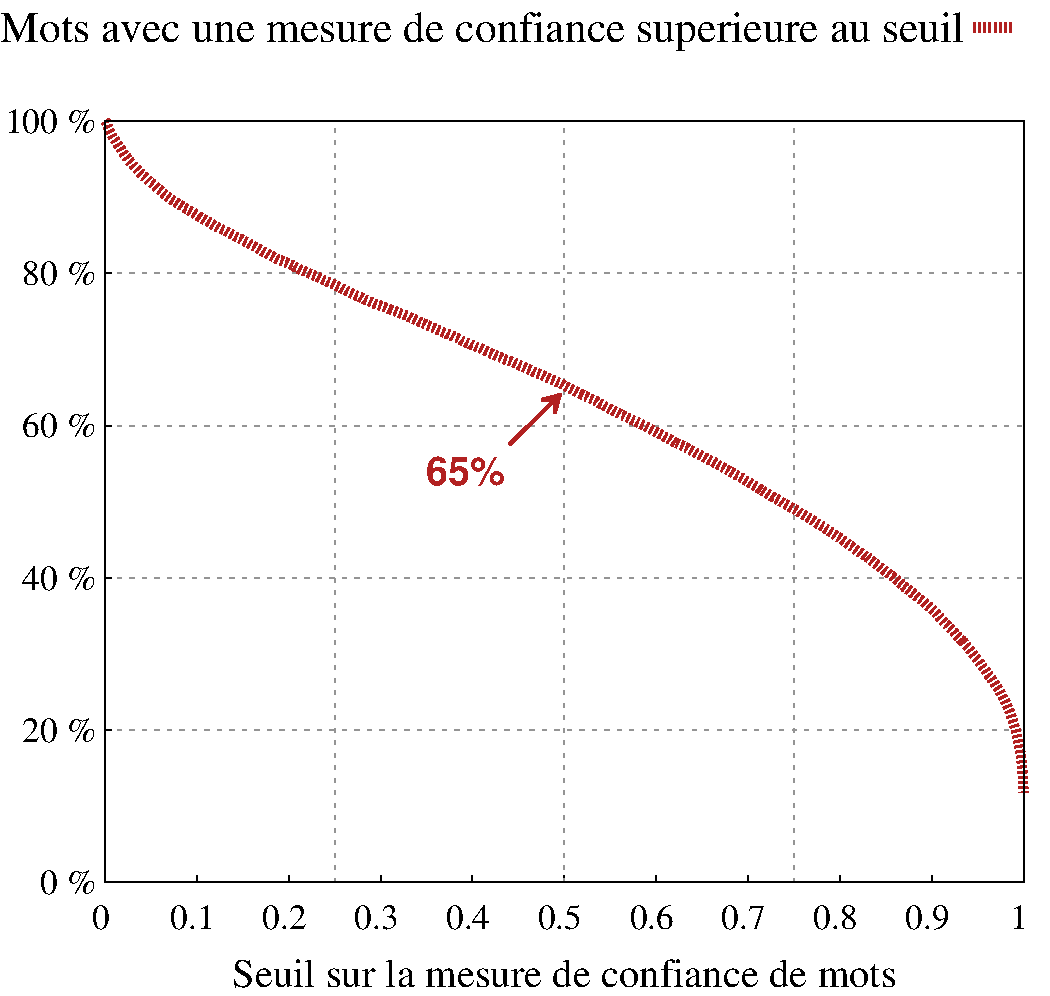
\includegraphics[scale=0.33]{Image/results/ESTER_combined_min3occ_words_CM_c1.pdf}
	\end{center}

}

\only<2|handout:0>
{
	\begin{center}
	\vskip-0.5ex
	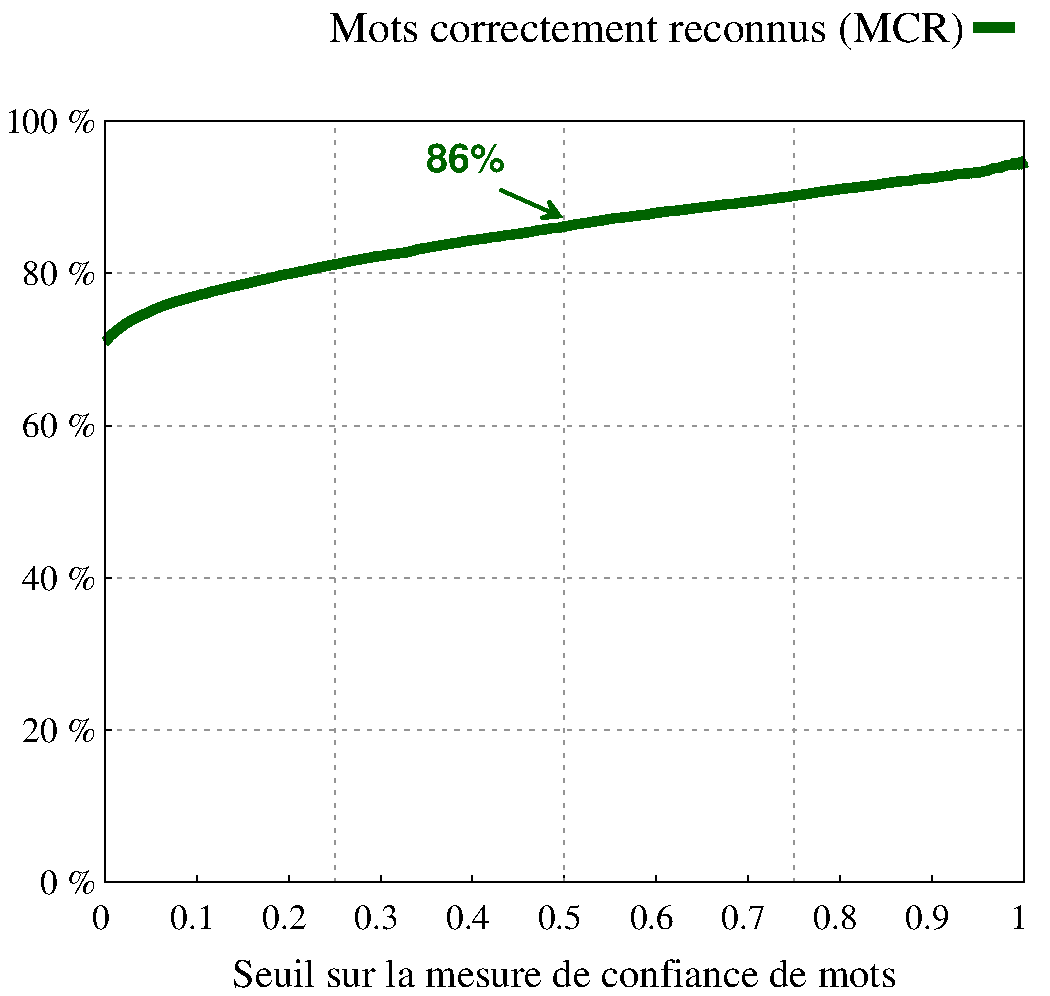
\includegraphics[scale=0.33]{Image/results/ESTER_combined_min3occ_words_CM_c2.pdf}
	\end{center}
}

\only<3->
{
	\begin{center}
	\vskip-0.5ex
	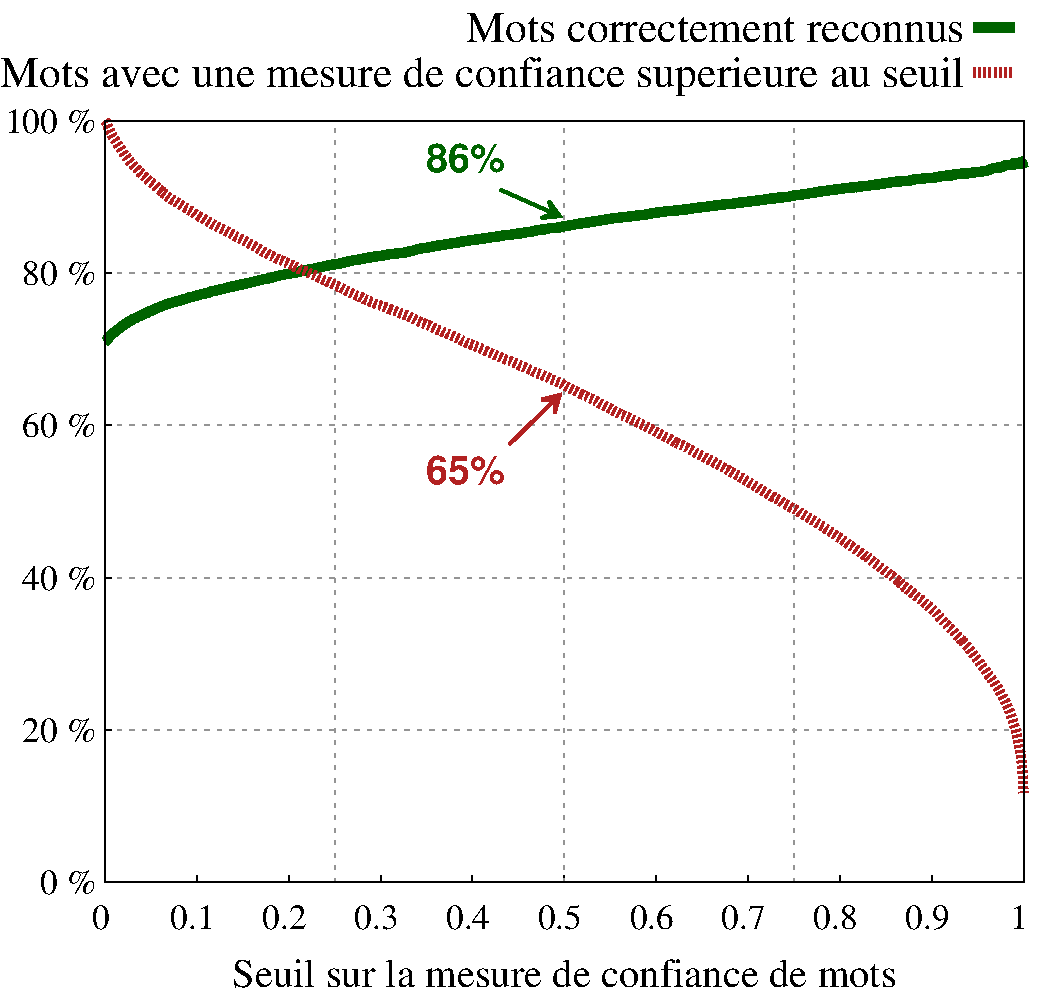
\includegraphics[scale=0.33]{Image/results/ESTER_combined_min3occ_words_CM.pdf}
	\end{center}
}

\end{column}
\begin{column}{0.15\textwidth}
\end{column}
\end{columns}

\vskip3ex

\only<1|handout:0>
{
\scriptsize {\color{darkcerulean}$\Rightarrow$} 65\% de mots ont une mesure de confiance supérieure à 0,5
}

\only<2|handout:0>
{
\scriptsize {\color{darkcerulean}$\Rightarrow$} 86\% de mots qui ont une mesure de confiance supérieure à 0,5 sont correctement reconnus
}

\only<3->
{
\scriptsize
{\color{darkcerulean}$\Rightarrow$} les mesures de confiance sur les mots sont pertinentes \\\vskip1ex
{\color{darkcerulean}$\Rightarrow$} 65\% mots MC $\ge$ 0,5 dont 86\% sont correctement reconnus\\\vskip1ex
}

\end{frame}


%==============================================================================================================
\subsection*{Conclusions}
\begin{frame}[t]{Conclusions sur les modèles hybrides}

{\footnotesize
\begin{itemize}

\vskip5ex
\item notre solution de modélisation hybride \\prend en compte les \textbf{\color{purple}prononciations réelles}

\vskip3ex
\item les sorties de reconnaissance contiennent essentiellement des mots

\vskip3ex
\item plus de 70\% de mots sont correctement reconnus

\vskip3ex
\item les mesures de confiance sont pertinentes \\pour selectionner les mots bien reconnus
%65\% de mots ont une mesure de confiance supérieure à 0,5 \\et parmi eux 86\% sont correctement reconnus

\vskip3ex
\item une quantité plus grande de syllabes dans le corpus d'apprentissage
	\begin{itemize}
	\vskip0.3ex \item  améliore le taux de syllabes correctement reconnues
	\vskip0.3ex \item  améliore le taux de mots hors-vocabulaire décodés par des syllabes
	\end{itemize}
\end{itemize}
}

\end{frame}




%==============================================================================================================
\section{Ajout de nouveaux mots}
\subsection*{Problématique et approche}
\begin{frame}[t]{Ajout de nouveaux mots}

\begin{itemize}
\vskip5ex
\item \textbf{\color{purple}Problématique}
	\begin{itemize}
	\vskip2ex
	\item mots hors-vocabulaire fréquemment prononcés
		\begin{itemize}
		\vskip1ex
		\item ex: mots spécifiques à un certain domaine
		\end{itemize}
	\end{itemize}

\vskip4ex
\item \textbf{\color{purple}L'ajout d'un nouveau mot implique}
	\begin{itemize}
	\vskip2ex
	\item la génération des variantes de prononciations
	\vskip2ex
	\item la modification du modèle de langage
	\end{itemize}

\end{itemize}



\end{frame}
%==============================================================================================================
\begin{frame}[t]{État de l'art : ajout de mots}

{\footnotesize
\begin{itemize}

\vskip3ex
\item adaptation du modèle de langage {\fontfamily{qcs}\selectfont \tiny \color{blendedblue} [DeMori et Federico 1999 ; Bellegarda 2004]}

\vskip3ex
\item utilisation des modèles de langage basés sur des classes \\{\fontfamily{qcs}\selectfont \tiny \color{blendedblue} [Brown et al. 1992 ; Suhm et Waibel 1994]}
	\begin{itemize}
	\vskip1.7ex
	\item {\scriptsize mots associés à une classe par rapport à des étiquettes morphologiques \\\vskip-0.3ex {\fontfamily{qcs}\selectfont \tiny \color{blendedblue} [Prazak et al. 2007]}}

	\vskip2ex
	\item {\scriptsize mots associés à leur classe grammaticale \\\vskip-0.3ex{\fontfamily{qcs}\selectfont \tiny \color{blendedblue} [Allauzen et Gauvain 2005, Martins et al. 2008]}}

	\vskip2ex
	\item {\scriptsize mots associés à la classe de leurs mots similaires (mesure du cosinus \\\vskip-0.3ex entre les vecteurs représentant les mots) {\fontfamily{qcs}\selectfont \tiny \color{blendedblue} [Naptali et al. 2012]}}
	\end{itemize}

%\vskip1.3ex
%\item fréquences de 2-grams inconnus estimées sur données disponibles sur internet  {\fontfamily{qcs}\selectfont \tiny \color{blendedblue} [Keller et Lapata 2003]}

\vskip3ex
\item chercher une liste des n-grammes représentant les nouveaux mots et calculer les probabilités de ces nouveaux n-grammes en se basant sur les probabilités des n-grammes connus  {\fontfamily{qcs}\selectfont \tiny \color{blendedblue} [Lecorve et al. 2011]}

\end{itemize}
}

\end{frame}



%==============================================================================================================
\begin{frame}[t]{Approche proposée}

\begin{itemize}
\vskip3ex
\item sans réapprentissage ou adaptation du modèle de langage
	\begin{itemize}
	\vskip1ex
	\item[$\rightarrow$] nécessite beaucoup de données relatives aux nouveaux mots
	\end{itemize}
\vskip4ex
\item basée sur la \textbf{\color{purple}similarité entre mots}

	\vskip1ex
	\begin{center}
	\hspace{-0.2cm}\begin{beamerboxesrounded}[width=0.79\textwidth,shadow=false]{}
		{\scriptsize
		\begin{tabular}{rcl}
			on ignorait encore lundi & \hskip-1.7ex \textbf{\color{purple}soir}  & \hskip-1.7ex les conditions de sa survie \\
			on ignorait encore lundi & \hskip-1.7ex \textbf{\color{ngreen}matin} & \hskip-1.7ex les conditions de sa survie \\
		\end{tabular}
		}
	\end{beamerboxesrounded}
	\end{center}

	\only<2->
	{
		\begin{itemize}
		\item[$\rightarrow$] utiliser \textbf{\color{blendedblue}quelques phrases exemples} \\pour chaque nouveau mot
		\vskip2ex
		\item[$\rightarrow$] trouver les mots connus similaires \\(\textbf{\color{blendedblue}distributions similaires des voisins})
		\vskip2ex
		\item[$\rightarrow$] \textbf{\color{blendedblue}transposer les probabilités} n-grammes des mots similaires \\sur les nouveaux mots
		\end{itemize}
	}
\end{itemize}


\end{frame}


%==============================================================================================================
\begin{frame}[t]{Voisins de nouveaux mots}

\begin{itemize}
\vskip-1ex
\item[\textbf{\color{blendedblue}1.}] Utilise quelques \textbf{\color{blendedblue}phrases exemples} avec le nouveau mot

	{\footnotesize
	\vskip1ex \hskip-0.5ex $\rightarrow$ calcule les distributions des voisins du nouveau mot \textbf{\color{purple}nW}
	\begin{center}$P_k(w|\textbf{\color{purple}nW}) \text{ pour } k \in \{..., -2, -1, +1, +2, ...\}$\end{center}
	}
\end{itemize}

\vskip1ex

\only<2->
{
\footnotesize
\vskip-1ex{\color{darkcerulean}\rule{\textwidth}{0.9pt}}

\begin{itemize}

\vskip-1ex
\item exemple de nouveau mot : \textbf{\color{purple}soir}

\vspace*{1ex}
\item phrases exemples

	\vspace*{-2.5ex}
	\begin{center}
	{\scriptsize
	\hspace*{-4ex}\begin{tabular}{rcccccl}
	 	   	   & {\color{blendedblue}$-2$} & {\color{blendedblue}$-1$} & & {\color{blendedblue}$+1$}  & {\color{blendedblue}$+2$}  & 	\\\cline{2-6}
	on ignorait 	   & \underline{encore} & \underline{lundi} 	& \textbf{\color{purple}soir} & \underline{les} & \underline{conditions} & de sa survie \\
	devine qui vient   & \underline{dîner}  & \underline{ce}    	& \textbf{\color{purple}soir} & & &  \\
	pas de consigne de & \underline{vote} 	& \underline{au} 	& \textbf{\color{purple}soir} & \underline{du}  & \underline{premier} 	 & tour \\
	\end{tabular}
	}
	\end{center}

\vspace*{1ex}
\item voisins prédécesseurs et successeurs \hskip0.5ex
	{\scriptsize
	\begin{tabular}{l|l}
	$k= -2$  	& encore, dîner, vote,  ... 	\\
	$k= -1$  	& lundi, ce, au, ... 		\\
	$k= +1$  	& les, du, ...    		\\
	$k= +2$  	& conditions, premier, ... 	\\
	\end{tabular}
	}

\end{itemize}

}

\end{frame}

%==============================================================================================================
\begin{frame}[t]{Voisins de mots connus}

\begin{itemize}
\vskip-1ex
\item[\textbf{\color{blendedblue}2.}] Cherche les mots similaires dans un \textbf{\color{blendedblue}corpus de référence}

	{\footnotesize
	\vskip1ex\hskip-0.5ex $\rightarrow$ calcule les distributions des voisins de chaque mot connu \textbf{\color{ngreen}kW}
	\begin{center}$P_k(w'|\textbf{\color{ngreen}kW}) \text{ for } k \in \{..., -2, -1, +1, +2, ...\}$\end{center}
	}
\end{itemize}

\vskip0.3ex

\only<2->
{
\footnotesize
\vskip-1ex{\color{darkcerulean}\rule{\textwidth}{0.9pt}}

\begin{itemize}
\item utilise directement le fichier de compteurs des séquences n-grammes
	\begin{itemize}
	\vspace*{0.1ex}
	\item {\scriptsize 3-gram $\Rightarrow$ maximum 4 voisins $k \in \{-2,-1,+1,+2\}$}
	\end{itemize}

\vspace*{2ex}
\item exemples des entrées 3-gram avec le mot connu `\textbf{\color{ngreen}matin}'

	\vskip1ex
	\begin{columns}
	\begin{column}{0.5\textwidth}
		{\scriptsize\fontfamily{qcr}\selectfont
		\renewcommand{\arraystretch}{1.01}
		\begin{tabular}{cccr}
		\hskip3ex "\textbf{\color{ngreen}matin} 	& a 				& été 				& \textit{10}" 	\\
		\hskip3ex "beau 				& \textbf{\color{ngreen}matin} 	& de 				& \textit{9}" 	\\
		\hskip3ex "jusqu' 				& au 				& \textbf{\color{ngreen}matin} 	& \textit{28}" 	\\
		\end{tabular}
		}
	\end{column}
	\begin{column}{0.5\textwidth}
		\vskip-1ex
		{\tiny
		\renewcommand{\arraystretch}{1.5}
		\begin{tabular}{ll}
		$\rightarrow$ voisin $k=+1$ `a'; 	& \hskip-3ex voisin $k=+2$ `été' 	\\
		$\rightarrow$ voisin $k=-1$ `beau'; 	& \hskip-3ex voisin $k=+1$ `de' 	\\
		$\rightarrow$ voisin $k=-2$ `jusqu'; 	& \hskip-3ex voisin $k=-1$ `au'
		\end{tabular}
		}
	\end{column}
	\end{columns}


\vspace*{2ex}
\item voisins prédécesseurs et successeurs \hskip1ex
	{\scriptsize
	\begin{tabular}{l|l}
	$k= -2$  	& jusqu', ... 		\\
	$k= -1$  	& beau, au, ... 	\\
	$k= +1$  	& de, a, ...    	\\
	$k= +2$  	& été, ... 		\\
	\end{tabular}
	}
\end{itemize}

}

\end{frame}


%==============================================================================================================
\begin{frame}[t]{Similarité entre mots}


\begin{itemize}
\vskip3ex
\item[\textbf{\color{blendedblue}3.}] Calcule la \textbf{\color{blendedblue}divergence KL} entre les distributions de voisins \\
	{\footnotesize \vskip2ex$\rightarrow$  entre chaque mot connu (\textbf{\color{ngreen}kW}) et un nouveau mot (\textbf{\color{purple}nW})}

	\vskip3ex
	\begin{center}
	\hspace{-0.2cm}\begin{beamerboxesrounded}[width=0.93\textwidth,shadow=false]{divergence calculé sur chaque position $k$}
		{\scriptsize
		\renewcommand{\arraystretch}{1.5}
		\begin{tabular}{rp{0.01cm}l}
		\hskip-0.3ex $D_{KL} \left( \ P_{k}(\bullet|\textbf{\color{ngreen}kW}) \ || \ {P_{k}(\bullet|\textbf{\color{purple}nW})}\ \right)$
		& \hskip-2ex =
		& \hskip-2ex $\sum\limits_{w \in V(\textbf{\color{purple}nW})}^{ } \ P_{k}(w|\textbf{\color{ngreen}kW}) \ log \left( \frac{P_{k}(w|\textbf{\color{ngreen}kW})}{P_{k}(w|\textbf{\color{purple}nW})} \right)$ \\
		\end{tabular}
		}
	\end{beamerboxesrounded}
	\end{center}

	\vskip3ex
	\begin{center}
	\hspace{-0.2cm}\begin{beamerboxesrounded}[width=0.93\textwidth,shadow=false]{divergence globale}
		\vskip0.8ex
		\begin{center}
		{\scriptsize $D(\textbf{\color{ngreen}kW},\textbf{\color{purple}nW})\ =\ \sum\limits_{k} D_{k}(\textbf{\color{ngreen}kW},\textbf{\color{purple}nW})$}
		\end{center}
	\end{beamerboxesrounded}
	\end{center}
\end{itemize}

\end{frame}

%==============================================================================================================
\begin{frame}[t]{Similarité entre mots}


\begin{itemize}
\vskip3ex
\item[\textbf{\color{blendedblue}4.}] Sélectionne \textbf{\color{blendedblue}les mots les plus similaires} au nouveau mot
	{\footnotesize \vskip1ex \hskip3ex $\rightarrow$ ceux ayant des divergences minimales}
\end{itemize}

\vskip3ex
\only<2->
{
	\begin{center}
	\hspace{-0.2cm}\begin{beamerboxesrounded}[width=0.9\textwidth,shadow=false]{}
		{\scriptsize {\color{purple}Exemples de mots similaires :} }

		\vskip0.9ex
		{\scriptsize
		\begin{tabular}{p{1.3cm}p{0.5cm}p{7cm}}
		& soir		& $\rightarrow$ \ matin, midi, dimanche, samedi, vendredi	\\
		& soirs		& $\rightarrow$ \ temps, joueurs, matchs, pays, matches	 	\\
		\end{tabular}
		}

		\vskip-1ex
		{\scriptsize
		\begin{tabular}{p{0.005cm}p{1.8cm}p{7cm}}
		& gouvernement 	& $\rightarrow$ \ parti, président, peuple, roi, mouvement 	\\
		& gouvernements	& $\rightarrow$ \ ministres, partis, syndicats, services, pays	\\
		\end{tabular}
		}
	\end{beamerboxesrounded}
	\end{center}
}

\end{frame}


%==============================================================================================================
\begin{frame}[t]{Ajout des n-grammes}

\begin{itemize}

\vspace*{-1ex}
\item[\textbf{\color{blendedblue}5.}] \textbf{\color{blendedblue}Transpose les probabilités} n-grammes des mots similaires \\ \hskip2ex sur les nouveaux mots

	\begin{itemize}
	\vskip1.5ex
	\item[$\rightarrow$] cherche les n-grammes qui contiennent les mots similaires

	\vskip1ex
	\item[$\rightarrow$] remplace les 'mots similaires' par le 'nouveau mot'

	\vskip1ex
	\item[$\rightarrow$] ajoute les nouveau n-grammes dans le nouveau modèle de langage
	\end{itemize}
\end{itemize}

\vskip0.1cm

\only<2->
{
\footnotesize
\vskip-1ex{\color{darkcerulean}\rule{\textwidth}{0.9pt}}


\begin{itemize}
\smallskip
\item nouveau mot "\textbf{\color{purple}soir}" similaire au mot connu "\textbf{\color{ngreen}matin}"

\vskip2ex
\item \underline{n-grammes connus}  (dans le modèle de langage) \\
	{\scriptsize
	\vskip1ex\hskip5ex {\scriptsize\fontfamily{qcr}\selectfont"-1.48214 possible ce \textbf{\color{ngreen}matin}"} \\
	\vskip1ex\hskip5ex {\scriptsize\fontfamily{qcr}\selectfont"-1.404164 \textbf{\color{ngreen}matin} ajoute que"}
	}

\vskip2ex
\item \underline{nouveaux n-grammes} (à ajouter dans le nouveau modèle de langage) \\
	{\scriptsize
	\vskip1ex\hskip5ex {\scriptsize\fontfamily{qcr}\selectfont"-1.48214 possible ce \textbf{\color{purple}soir}"} \\
	\vskip1ex\hskip5ex {\scriptsize\fontfamily{qcr}\selectfont"-1.404164 \textbf{\color{purple}soir} ajoute que"}
	}

\end{itemize}

}

\end{frame}




%==============================================================================================================
\subsection*{Expérimentations}
\begin{frame}[t]{Contexte expérimental}

\begin{itemize}
\vskip3ex
\item Sélectionne les nouveaux mots à ajouter dans le ML \\ \hskip1ex {\scriptsize $\Rightarrow$ \textbf{\color{purple}44 nouveaux mots} }

\vskip4ex
\item Configuration pour la recherche les mots similaires
	\begin{itemize}
	\vskip2ex
	\item {\scriptsize phrases basés sur les unités  "\textbf{\color{orange}mot}$|$classe grammaticale"}

		\vskip1ex
		\begin{columns}
		\begin{column}{0.1\textwidth}
		\end{column}
		\begin{column}{1.08\textwidth}
		\hspace*{2ex}
		\begin{beamerboxesrounded}[width=0.85\textwidth,shadow=false]{}
			{\scriptsize \textbf{\color{orange}qui}$|$PRO:REL \hskip1ex \textbf{\color{orange}vient}$|$VER:pres \hskip1ex \textbf{\color{orange}dîner}$|$VER:infi
			\hskip1ex \textbf{\color{orange}ce}$|$PRO:DEM \hskip1ex  \textbf{\color{orange}soir}$|$NOM }
		\end{beamerboxesrounded}
		\end{column}
		\end{columns}

	\vskip2ex
	\item {\scriptsize 4 voisins pour chaque mot : $k \in \{-2, -1, +1, +2\}$}
	\end{itemize}

\vskip4ex
\item Évaluer l'impact du
	\begin{itemize}
	\vskip1ex
	\item nombre de phrases exemples pour un nouveau mot {\scriptsize (5, 10, 20 ou 50) }
	\vskip0.5ex
	\item nombre de mots similaires pour un nouveau mot {\scriptsize (5, 10, 20 ou 50) }
	\end{itemize}
\end{itemize}

\end{frame}



%==============================================================================================================
\begin{frame}[t]{Contexte expérimental}

\begin{itemize}

\vskip1ex
\item modèle de langage \textbf{\color{purple}BASELINE}
	\begin{itemize}
	\vskip0.5ex
	\item {\scriptsize modèle grand vocabulaire appris par interpolation}
	\vskip0.1ex
	\item {\scriptsize les 44 nouveaux mots ne sont pas présents dans le modèle}
	\end{itemize}


\vskip2ex
\item modèle de langage \textbf{\color{purple}ORACLE}
	\begin{itemize}
	\vskip0.5ex
	\item {\scriptsize modèle grand vocabulaire appris par interpolation }
	\vskip0.1ex
	\item {\scriptsize les 44 nouveaux mots sont présents dans le modèle}
	\end{itemize}

\vskip2ex
\item 4 modèles de langage \textbf{\color{purple}LM-INTERP-1,-2,-3,-4}
	\begin{itemize}
	\vskip1ex
	\item {\scriptsize modèle grand vocabulaire appris par interpolation \\
		\vskip0.5ex\hskip1ex {\color{darkcerulean}-} sur les mêmes ensembles de données que `BASELINE' \\
		\vskip0.3ex\hskip1ex {\color{darkcerulean}-} plus les phrases exemples pour chaque nouveau mot (5, 10, 20 ou 50) }
	\vskip0.5ex
	\item {\scriptsize les 44 nouveaux mots sont présents dans le modèle}
	\end{itemize}

\end{itemize}

\vskip2ex
\hspace*{1.2ex}\begin{beamerboxesrounded}[width=0.97\textwidth,shadow=false]{}
{\footnotesize
{\color{darkcerulean}{\fontencoding{U}\fontfamily{futs}\selectfont\char 66\relax}}
poids optimaux d'interpolation estimés sur le corpus d'ETAPE (dév) \\
\hspace*{3ex} {\color{darkcerulean}$\rightarrow$} les 44 nouveaux mots ont une fréquence d'occurrence de 0,93\%
}
\end{beamerboxesrounded}



\end{frame}




%==============================================================================================================
\begin{frame}[t]{Taille des modèles}

\begin{itemize}
\vskip4ex
\item \textbf{\color{purple}Nouveaux modèles de langage} ({\footnotesize\color{blendedblue}'baseline+1-,2-,3-grams'})
	\begin{itemize}
	\vskip2ex
	\item en ajoutant des 1-,2-,3-grammes de nouveaux mots dans BASELINE

	\vskip2ex
	\item nouveaux n-grammes choisis en fonction du
		\begin{itemize}
		\vskip1.5ex
		\item nombre de phrases exemples par nouveau mot (5, 10, 20 ou 50)

		\vskip1ex
		\item nombre de mots similaires par nouveau mot (5, 10, 20 ou 50)
		\end{itemize}
	\end{itemize}
\end{itemize}

\vspace*{3ex}

\only<2|handout:0>
{
	\scriptsize
	\hspace*{-2ex}\begin{tabular}{|r|r|rr|rr|r|}
	\cline{2-7}
	\multicolumn{1}{c|}{} & \multirow{3}{*}{\textbf{baseline}} & \multicolumn{4}{c|}{\textbf{\color{purple}'baseline+1-,2-,3-grams'}} & \multirow{2}{*}{\textbf{ORACLE}} \\ \cline{3-6}
	\multicolumn{1}{c|}{} 	& 		& \multicolumn{2}{l|}{{\color{purple}5} phrases exemple} & \multicolumn{2}{l|}{{\color{purple}50} phrases exemple} &	\\
	\multicolumn{1}{c|}{} 	& 		& \multicolumn{2}{l|}{{\color{purple}5} mots similaires} & \multicolumn{2}{l|}{{\color{purple}50} mots similaires} &	\\ \hline
	\#2-grams  		& 37,1		& 38,0 & {\color{blue}[+2\%]}	& &	& 43,3	\\
	\#3-grams		& 63,1		& 67,2 & {\color{blue}[+6\%]}	& &	& 80,1	\\ \hline
	\end{tabular}
	\vskip2ex\begin{center}{\scriptsize Nombre [en millions] de 2-grams et de 3-grams}\end{center}
}

\only<3->
{
	\scriptsize
	\hspace*{-2ex}\begin{tabular}{|r|r|rr|rr|r|}
	\cline{2-7}
	\multicolumn{1}{c|}{} & \multirow{3}{*}{\textbf{baseline}} & \multicolumn{4}{c|}{\textbf{\color{purple}'baseline+1-,2-,3-grams'}} & \multirow{2}{*}{\textbf{ORACLE}} \\ \cline{3-6}
	\multicolumn{1}{c|}{} 	& 		& \multicolumn{2}{l|}{{\color{purple}5} phrases exemple} & \multicolumn{2}{l|}{{\color{purple}50} phrases exemple} &	\\
	\multicolumn{1}{c|}{} 	& 		& \multicolumn{2}{l|}{{\color{purple}5} mots similaires} & \multicolumn{2}{l|}{{\color{purple}50} mots similaires} &	\\ \hline
	\#2-grams  		& 37,1		& 38,0 & {\color{blue}[+2\%]}	& 40,7 & {\color{blue}[+10\%]}	& 43,3	\\
	\#3-grams		& 63,1		& 67,2 & {\color{blue}[+6\%]}	& 94,2 & {\color{blue}[+49\%]}	& 80,1	\\ \hline
	\end{tabular}
	\vskip2ex\begin{center}{\scriptsize Nombre [en millions] de 2-grams et de 3-grams}\end{center}
}
\end{frame}



%==============================================================================================================
\begin{frame}[t]{Évaluation de l'approche}

\begin{itemize}

\vskip6ex
\item Expérimentations
	\begin{itemize}
	\vskip2ex
	\item les ML sont évalués sur l'ensemble de développement d'ESTER2
	\vskip2ex
	\item les 44 nouveaux mots ont une fréquence d'occurrence de 1,33\%
	\end{itemize}

\vskip5ex
\item Compare les performances des modèles de langage
	\begin{itemize}
	\vskip2ex
	\item taux d'erreur mot (WER)
	\vskip2ex
	\item taux de nouveaux mots correctement reconnus
	\end{itemize}
\end{itemize}

\end{frame}



%==============================================================================================================
\begin{frame}[t]{Taux d'erreur mot (WER)}

\vspace*{-2ex}
\begin{columns}
\begin{column}{0.4\textwidth}
\begin{table}[h]
\footnotesize
\begin{tabular}{rl}
BASELINE  	& \textbf{\color{blendedblue}26,97\%}  \\
ORACLE  	& \textbf{\color{blendedblue}24,80\%} \\
\end{tabular}
\end{table}
\end{column}
\begin{column}{0.5\textwidth}
\only<1>
{
	\begin{beamerboxesrounded}[width=0.7\textwidth,shadow=false]{}
	\centering
		{\scriptsize{\color{darkcerulean}{\fontencoding{U}\fontfamily{futs}\selectfont\char 66\relax}}
		1,33\% d'occurrences \\des 44 nouveaux mots}
	\end{beamerboxesrounded}
}
\end{column}
\end{columns}

\vspace*{-2.7ex}

\only<2|handout:0>
{
\begin{center}
\begin{table}[h]
\scriptsize
\renewcommand{\arraystretch}{1.3}
\begin{tabular}{c|c|c||r|r|r|r|}
\cline{3-7}
\multicolumn{1}{c}{} & \multicolumn{1}{c|}{} & \multirow{3}{*}{\textbf{\footnotesize LM-INTERP}} & \multicolumn{4}{c|}{\textbf{\footnotesize `baseline+1-,2-,3-grams'}}	\\ \cline{4-7}
\multicolumn{1}{c}{} & \multicolumn{1}{c|}{} & 			 & \multicolumn{4}{c|}{\# de mots similaires}		\\
\multicolumn{1}{c}{} & \multicolumn{1}{c|}{} & 			 & \multicolumn{1}{c}{5} & \multicolumn{1}{c}{10} & \multicolumn{1}{c}{20} & \multicolumn{1}{c|}{50} \\ \cline{2-7}
\parbox[t]{2mm}{\multirow{4}{*}{\rotatebox[origin=c]{90}{\# phrases}}} \parbox[t]{2mm}{\multirow{4}{*}{\rotatebox[origin=c]{90}{exemples}}}
	& 5   	& 				& {\bf 25,78}	& 25,83	& 25,96	& 26,01			\\ \cline{2-2}\cline{4-7}
	& 10   	& 				& {\bf 25,74}	& 25,84 & 25,96	& 26,05			\\ \cline{2-2}\cline{4-7}
	& 20 	& 				& {\bf {\color{red}25,63}}	& 25,68	& 25,92	& 25,95			\\ \cline{2-2}\cline{4-7}
	& 50 	& 				& {\bf 25,68}	& 25,75	& 25,82	& 25,99			\\ \cline{2-2}\cline{2-7}
\end{tabular}
\end{table}
\end{center}


{\scriptsize
\vskip1ex\hskip-1ex {\color{darkcerulean}$\Rightarrow$} des meilleures performances sont obtenues avec \textbf{\color{purple}peu de mots similaires} (5) \\et avec un \textbf{\color{purple}nombre raisonnable de phrases exemples} (20-50)

\vskip3ex\hskip-1ex {\color{darkcerulean}$\Rightarrow$} l'ajout de n-grammes pour les nouveaux mots fournit une \\\textbf{\color{purple}amélioration absolue de 1,3\%} sur le taux d'erreur mot
}
}


\only<3>
{
\begin{center}
\begin{table}[h]
\scriptsize
\renewcommand{\arraystretch}{1.3}
\begin{tabular}{c|c|c||r|r|r|r|}
\cline{3-7}
\multicolumn{1}{c}{} & \multicolumn{1}{c|}{} & \multirow{3}{*}{\textbf{\footnotesize LM-INTERP}} & \multicolumn{4}{c|}{\textbf{\footnotesize `baseline+1-,2-,3-grams'}}	\\ \cline{4-7}
\multicolumn{1}{c}{} & \multicolumn{1}{c|}{} & 	& \multicolumn{4}{c|}{\# de mots similaires}		\\
\multicolumn{1}{c}{} & \multicolumn{1}{c|}{} & 	& \multicolumn{1}{c}{5} & \multicolumn{1}{c}{\color{lightgray}10} & \multicolumn{1}{c}{\color{lightgray}20} & \multicolumn{1}{c|}{\color{lightgray}50} \\ \cline{2-7}
\parbox[t]{2mm}{\multirow{4}{*}{\rotatebox[origin=c]{90}{\# phrases}}} \parbox[t]{2mm}{\multirow{4}{*}{\rotatebox[origin=c]{90}{exemples}}}
	& 5   	& 26,12				& {\bf 25,78}	& {\color{lightgray}25,83} & {\color{lightgray}25,96}	& {\color{lightgray}26,01}	\\ \cline{2-7}
	& 10   	& 26,02				& {\bf 25,74}	& {\color{lightgray}25,84} & {\color{lightgray}25,96}	& {\color{lightgray}26,05}	\\ \cline{2-7}
	& 20 	& 25,81				& {\bf {\color{red}25,63}}	& {\color{lightgray}25,68} & {\color{lightgray}25,92}	& {\color{lightgray}25,95}	\\ \cline{2-7}
	& 50 	& 25,68				& {\bf 25,68}	& {\color{lightgray}25,75} & {\color{lightgray}25,82}	& {\color{lightgray}25,99}	\\ \cline{2-7}
\end{tabular}
\end{table}
\end{center}

{\scriptsize
\vskip1ex\hskip-1ex {\color{darkcerulean}$\Rightarrow$} les modèles `baseline+1-,2-,3-grams' surpassent les modèles 'LM-INTERP'
}
}

\end{frame}

%==============================================================================================================
\begin{frame}[t]{Taux de nouveaux mots bien reconnus}

\vspace*{-2ex}
\begin{columns}
\begin{column}{0.4\textwidth}
\begin{table}[h]
\footnotesize
\begin{tabular}{rr}
BASELINE  	& \textbf{\color{blendedblue}0,00\%}  \\
ORACLE  	& \textbf{\color{blendedblue}85,45\%} \\
\end{tabular}
\end{table}
\end{column}
\begin{column}{0.5\textwidth}
\end{column}
\end{columns}


\vspace*{-2.7ex}

\only<2|handout:0>
{

\begin{center}
\begin{table}[h]
\scriptsize
\renewcommand{\arraystretch}{1.3}
\begin{tabular}{c|c|c||r|r|r|r|}
\cline{3-7}
\multicolumn{1}{c}{} & \multicolumn{1}{c|}{} & \multirow{3}{*}{\textbf{\footnotesize LM-INTERP}} & \multicolumn{4}{c|}{\textbf{\footnotesize `baseline+1-,2-,3-grams'}}	\\ \cline{4-7}
\multicolumn{1}{c}{} & \multicolumn{1}{c|}{} & 				  & \multicolumn{4}{c|}{\# de mots similaires}		\\
\multicolumn{1}{c}{} & \multicolumn{1}{c|}{} & 			 & \multicolumn{1}{c}{5} & \multicolumn{1}{c}{10} & \multicolumn{1}{c}{20} & \multicolumn{1}{c|}{50} \\ \cline{2-7}
\parbox[t]{2mm}{\multirow{4}{*}{\rotatebox[origin=c]{90}{\# phrases}}} \parbox[t]{2mm}{\multirow{4}{*}{\rotatebox[origin=c]{90}{exemples}}}
	& 5   	& 				& {\bf 64,90}	& 61,09	& 58,36	& 56,72			\\ \cline{2-2}\cline{4-7}
	& 10   	& 				& {\bf 63,09}	& 61,09	& 57,09	& 55,27			\\ \cline{2-2}\cline{4-7}
	& 20 	& 				& {\bf {\color{red}68,72}}	& 65,81	& 61,27	& 58,18			\\ \cline{2-2}\cline{4-7}
	& 50 	& 				& {\bf 68,54}	& 63,45	& 61,81	& 57,09			\\ \cline{2-2}\cline{2-7}
\end{tabular}
\end{table}
\end{center}

{\scriptsize
\vskip1ex\hskip-1ex {\color{darkcerulean}$\Rightarrow$} des meilleures performances sont obtenues avec \textbf{\color{purple}peu de mots similaires} (5) \\et avec un \textbf{\color{purple}nombre raisonnable de phrases exemples} (20-50)

\vskip3ex\hskip-1ex {\color{darkcerulean}$\Rightarrow$} l'ajout de n-grammes pour les nouveaux mots permet de \\\textbf{\color{purple}reconnaître correctement 69\% des nouveaux mots}
}
}

\only<3->
{

\begin{center}
\begin{table}[h]
\scriptsize
\renewcommand{\arraystretch}{1.3}
\begin{tabular}{c|c|c||r|r|r|r|}
\cline{3-7}
\multicolumn{1}{c}{} & \multicolumn{1}{c|}{} & \multirow{3}{*}{\textbf{\footnotesize LM-INTERP}} & \multicolumn{4}{c|}{\textbf{\footnotesize `baseline+1-,2-,3-grams'}}	\\ \cline{4-7}
\multicolumn{1}{c}{} & \multicolumn{1}{c|}{} & 				  & \multicolumn{4}{c|}{\# de mots similaires}		\\
\multicolumn{1}{c}{} & \multicolumn{1}{c|}{} & 			 & \multicolumn{1}{c}{5} & \multicolumn{1}{c}{\color{lightgray}10} & \multicolumn{1}{c}{\color{lightgray}20} & \multicolumn{1}{c|}{\color{lightgray}50} \\ \cline{2-7}
\parbox[t]{2mm}{\multirow{4}{*}{\rotatebox[origin=c]{90}{\# phrases}}} \parbox[t]{2mm}{\multirow{4}{*}{\rotatebox[origin=c]{90}{exemples}}}
	& 5   	& 44,72				& {\bf 64,90}	& {\color{lightgray}61,09} & {\color{lightgray}58,36}	& {\color{lightgray}56,72}	\\ \cline{2-7}
	& 10   	& 47,45				& {\bf 63,09}	& {\color{lightgray}61,09} & {\color{lightgray}57,09}	& {\color{lightgray}55,27}	\\ \cline{2-7}
	& 20 	& 54,18				& {\bf {\color{red}68,72}}	& {\color{lightgray}65,81} & {\color{lightgray}61,27}	& {\color{lightgray}58,18}	\\ \cline{2-7}
	& 50 	& 59,63				& {\bf 68,54}	& {\color{lightgray}63,45} & {\color{lightgray}61,81}	& {\color{lightgray}57,09}	\\ \cline{2-7}
\end{tabular}
\end{table}
\end{center}


{\scriptsize
\vskip1ex\hskip-1ex {\color{darkcerulean}$\Rightarrow$} les modèles `baseline+1-,2-,3-grams' surpassent les modèles 'LM-INTERP'
}
}


\end{frame}


%==============================================================================================================
\subsection*{Conclusions}
\begin{frame}[t]{Conclusions sur l'ajout de nouveaux mots}

{\footnotesize
\begin{itemize}

\vskip5ex
\item notre approche d'utiliser la similarité entre mots pour \\\vskip1ex l'ajout de nouveaux n-grammes dans un modèle est efficace

\vskip4ex
\item l'ajout de n-grammes pour les nouveaux mots fournit \\\vskip1ex une amélioration absolue de \textbf{\color{blendedblue}1,3\%} sur le taux d'erreur mot \\\vskip1ex et permet de reconnaître correctement \textbf{\color{blendedblue}69\%} des nouveaux mots

\vskip4ex
\item les nouveaux modèles surpassent les modèles interpolés

\end{itemize}
}

\end{frame}






%==============================================================================================================
\section{Détection de questions}
\subsection*{Problématique et approche}
\begin{frame}[t]{Détection de questions}


{\scriptsize \textbf{\color{purple}Objectif} : déterminer à partir de la transcription automatique si la phrase \\\hskip11ex  est une question ou une affirmation}
%inform the deaf people if a question was directed to them

\bigskip
\begin{center}
\vskip-1.9ex
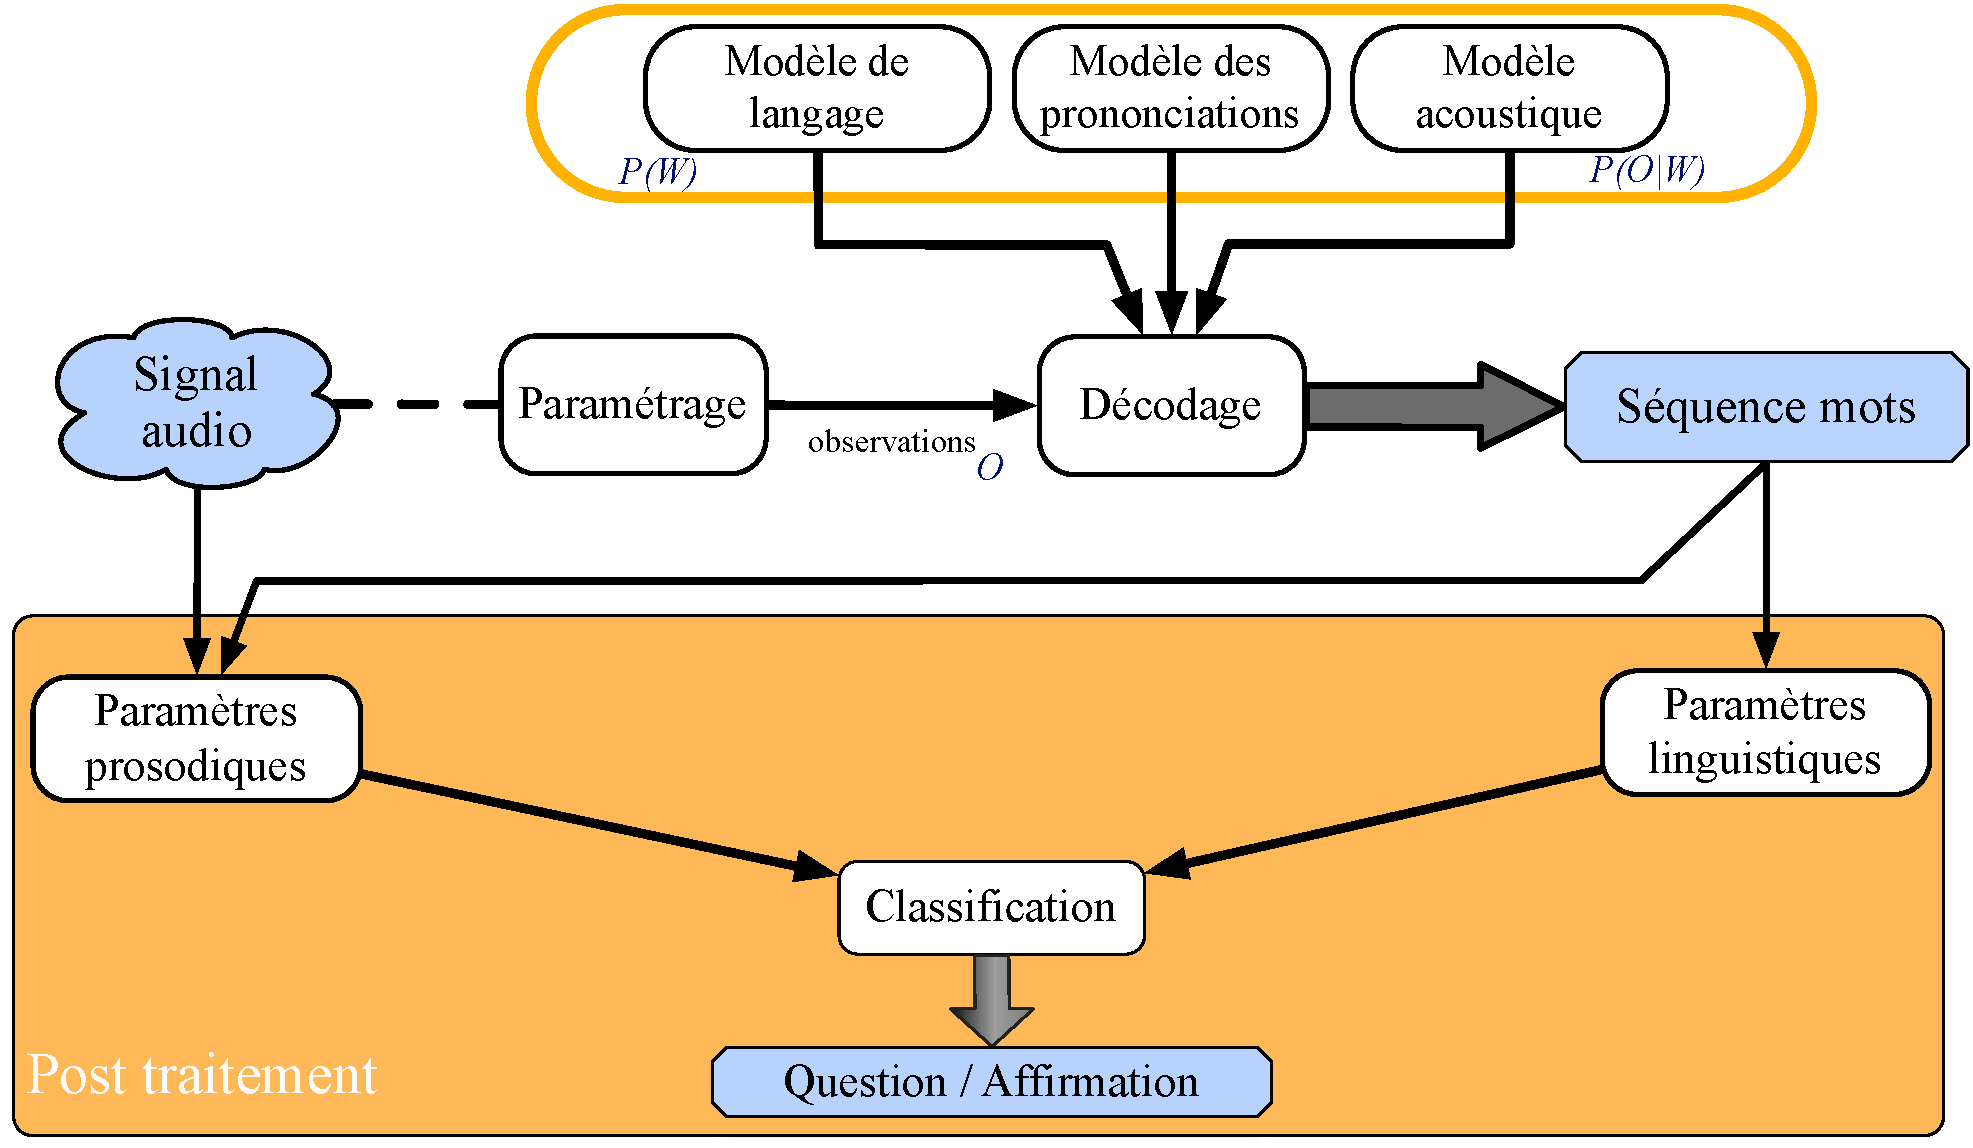
\includegraphics[scale=0.27]{Image/picture/rec_app_4.pdf}
\end{center}



\end{frame}


%==============================================================================================================
\begin{frame}[t]{État de l'art : détection de la modalité}

\begin{itemize}
{\footnotesize
\vskip1ex
\item \textbf{\color{purple}paramètres prosodiques}

	\begin{itemize}
	{\scriptsize
	\vskip1ex
	\item calculés sur les dernières 700ms du signal \\ {\scriptsize {\color{gray}(détection de questions, affirmations, exclamations françaises)}} {\fontfamily{qcs}\selectfont \tiny \color{blendedblue} [Kral et al. 2005]}\hspace*{-3ex}

	\vskip2ex
	\item calculés sur phrase complète \\ {\scriptsize {\color{gray}(détection de questions françaises)}} {\fontfamily{qcs}\selectfont \tiny \color{blendedblue} [Quang et al. 2006]}

	\vskip2ex
	\item calculés sur 3 parties du signal \\ {\scriptsize {\color{gray}(détection de questions arabes)}} {\fontfamily{qcs}\selectfont \tiny \color{blendedblue} [Khan et al. 2010]}
	}
	\end{itemize}

\vskip3ex
\item combinaison des \textbf{\color{purple}paramètres prosodiques et linguistiques}

	\begin{itemize}
	{\scriptsize
	\vskip1ex
	\item sur données correctes \\{\fontfamily{qcs}\selectfont \tiny \color{blendedblue} [Liscombe et al. 2006, Quang et al. 2007, Margolis et Ostendorf 2011]}

	\vskip2ex
	\item sur transcriptions automatiques \\{\fontfamily{qcs}\selectfont \tiny \color{blendedblue} [Jurafsky et al. 1997, Boakye et al. 2009, Kolar et Lamel 2012]}
	}
	\end{itemize}
}
\end{itemize}

\end{frame}


%==============================================================================================================
\begin{frame}[t]{Approche}

\begin{itemize}

\vskip-2ex
\item \textbf{\color{purple}classifieur prosodique}

	\vskip0.1ex\hskip0.8ex {\scriptsize {\color{darkcerulean}$\rightarrow$} phrases perçues comme questions par le biais de l'intonation}

		\vskip0.1ex
		\begin{center}
		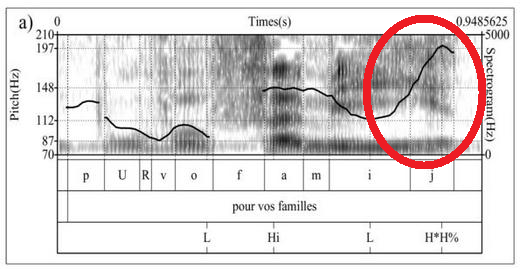
\includegraphics[scale=0.3]{Image/picture/prosodie_v2.png}
		\end{center}

\vspace*{-1ex}
\item \textbf{\color{purple}classifieur linguistique}

	\vskip0.1ex\hskip0.8ex {\scriptsize {\color{darkcerulean}$\rightarrow$} phrases perçues comme des questions par le biais de formes interrogatives}\hspace*{-3ex}

		\vskip1ex\hskip5ex\begin{beamerboxesrounded}[width=0.6\textwidth,shadow=false]{}
		\vskip0.1ex {\scriptsize {\color{darkcerulean}$\ast$} \textbf{\color{ngreen}qu'est ce qu}'on doit comprendre ?}
		\vskip0.4ex {\scriptsize {\color{darkcerulean}$\ast$} \textbf{\color{ngreen}est ce que} vous souhaitez une confrontation ?}
		\end{beamerboxesrounded}

\vskip2ex
\item \textbf{\color{purple}classifieur combiné} : utilise les deux types d'information
\end{itemize}

\end{frame}

%==============================================================================================================
\begin{frame}[t]{Paramètres prosodiques et linguistiques}

\begin{itemize}

\vspace*{-1ex}
\item<1-> 24 paramètres prosodiques calculés sur la phrase entière

	\begin{itemize}
	\vskip1ex
	\item 2 paramètres \textbf{\color{purple}généraux}

	\vskip1ex
	\item 4 paramètres liés à l'\textbf{\color{purple}énergie}

	\vskip1ex
	\item 18 paramètres liés à la \textbf{\color{purple}fréquence fondamentale} (F0)

	\end{itemize}

\vskip2ex
\item<2-> 3 paramètres linguistiques
	\begin{itemize}

	\vspace*{1ex}
	\item présence des motifs interrogatifs

		\vskip1ex\hskip5ex\begin{beamerboxesrounded}[width=0.8\textwidth,shadow=false]{}
		{\scriptsize
		quel, quelle, quels, quelles, comment, combien, pourquoi,
		\vskip0.3ex est ce que, est ce qu', qu' est ce, qu' est ce que, qu' est ce qu'}
		\end{beamerboxesrounded}

	\vskip2ex
	\item<3-> rapport de vraisemblance {\footnotesize (\textbf{\color{blendedblue} lexLLR, synLLR})}

	\vspace*{1ex}
	  	\begin{columns}
		\begin{column}{.13\textwidth}
		\end{column}
		\begin{column}{.67\textwidth}
		\vskip-4ex
		\scriptsize
		$$\text{LLR(phrase)}=\text{Log}\left(\frac{\text{P(phrase} \rvert \text{\color{ngreen}ML-question)}}{\text{P(phrase} \rvert \text{\color{orange}LM-affirmation)}}\right)$$
		\end{column}
		\begin{column}{.38\textwidth}
			\hskip1ex
\includegraphics[scale=0.13]{Image/picture/LM-qs-fr_v2.pdf}
		\end{column}
		\end{columns}

	\end{itemize}

\end{itemize}

\end{frame}



%=====================================================================================================================
\subsection*{Expérimentations}
\begin{frame}[t]{Contexte expérimental}

\begin{itemize}
\vskip4ex
\item Ensembles de \textbf{\color{purple}questions et affirmations}
	\begin{itemize}
	\vskip0.5ex
	\item extraits des corpus textuels en fonction de la ponctuation \textit{(?.)}
	\end{itemize}

\vskip4ex
\item Données pour \textbf{\color{purple}apprendre les modèles de langage}
	\begin{itemize}
	\vskip0.5ex
	\item corpus textuel GigaWord : \#89K questions, \#16M affirmations
	\end{itemize}

\vskip4ex
\item Données pour \textbf{\color{purple}apprendre et évaluer les classifieurs}
	\begin{itemize}
	\vskip0.5ex
	\item corpus audio Ester, Etape, Epac (transcrits manuellement)
	\end{itemize}
\end{itemize}


\vskip2ex
\begin{center}
	{\footnotesize
	\hskip-6ex\begin{tabular}{r|r|r}
			& \textbf{\#questions}	& \textbf{\#affirmations}	\\ \hline
	apprentissage 	& 10.5K			& 10.5K				\\
	évaluation  	&  0.9K			&  7.7K				\\
	\end{tabular}
	}
\end{center}

\end{frame}




%==============================================================================================================
\begin{frame}[t]{Classification question / affirmation}

\begin{itemize}
\vskip3ex
\item Classifieur à base de \textbf{\color{purple} règles de décision} {\footnotesize (JRip, outil WEKA)}

\vskip4ex
\item 2 configurations

	\begin{itemize}
	\vskip1ex
	\item {\scriptsize \textbf{\color{purple}transcriptions manuelles} (0\% taux d'erreur mot)}

	\vskip1ex
	\item {\scriptsize \textbf{\color{purple}transcriptions automatiques} (26\% taux d'erreur mot)}
	\end{itemize}

\vskip3ex
\item métrique de performance
	\vspace*{1.3ex}
	\begin{center}
		$\frac{1}{\text{H}}=\frac{1}{\text{2}} * \left(\frac{1}{\text{questionsCC}}  + \frac{1}{\text{affirmationsCC}}\right)$
	\end{center}

	\vspace*{1.3ex}{\scriptsize questionsCC \hskip2.4ex = pourcentage de questions correctement classées} \\
	\vskip0.2ex {\scriptsize affirmationsCC = pourcentage d'affirmations correctement classées}
\end{itemize}

\end{frame}



%==============================================================================================================
\begin{frame}[t]{Impact des transcriptions}

\begin{itemize}
\item {\footnotesize Classification sur transcriptions \textbf{\color{purple}manuelles} et \textbf{\color{purple}automatiques} }
\end{itemize}


\vskip0.2ex

\only<1>
{
\begin{center} 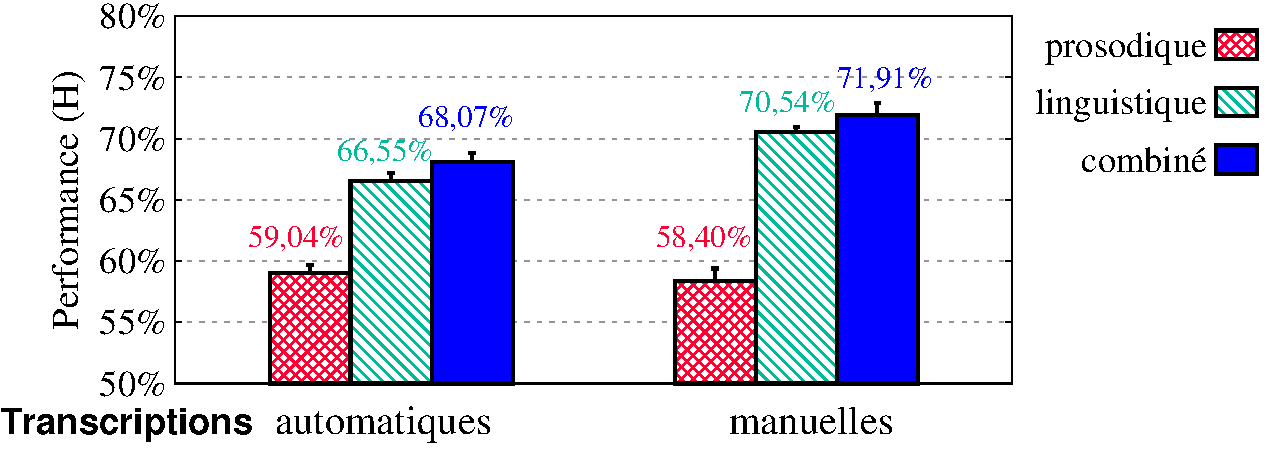
\includegraphics[scale=0.42]{Image/results/JRip_automatic_manual.pdf} \end{center}
}

\only<2|handout:0>
{
\begin{center} 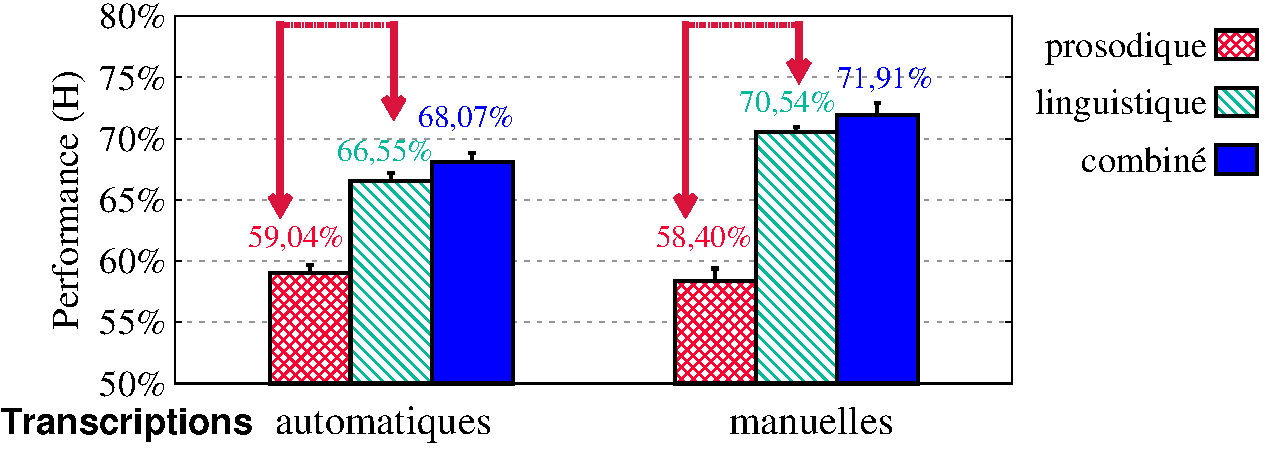
\includegraphics[scale=0.42]{Image/results/JRip_automatic_manual_v1.pdf} \end{center}

\vskip0.3ex
{\scriptsize {\color{purple}$\Rightarrow$} les classifieurs {\color{ngreen}linguistiques} surpassent les classifieurs  {\color{red}prosodiques}}
}

\only<3|handout:0>
{
\begin{center} 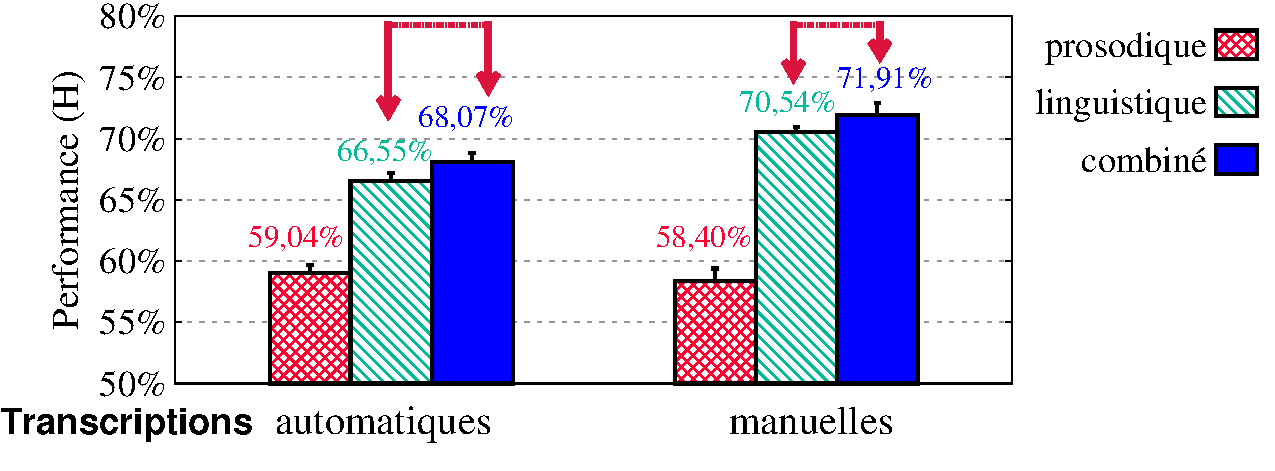
\includegraphics[scale=0.42]{Image/results/JRip_automatic_manual_v2.pdf} \end{center}

\vskip0.3ex
{\scriptsize {\color{purple}$\Rightarrow$} les classifieurs  {\color{blue}combinés} surpassent les classifieurs  {\color{ngreen}linguistiques} }
}

\only<4|handout:0>
{
\begin{center} 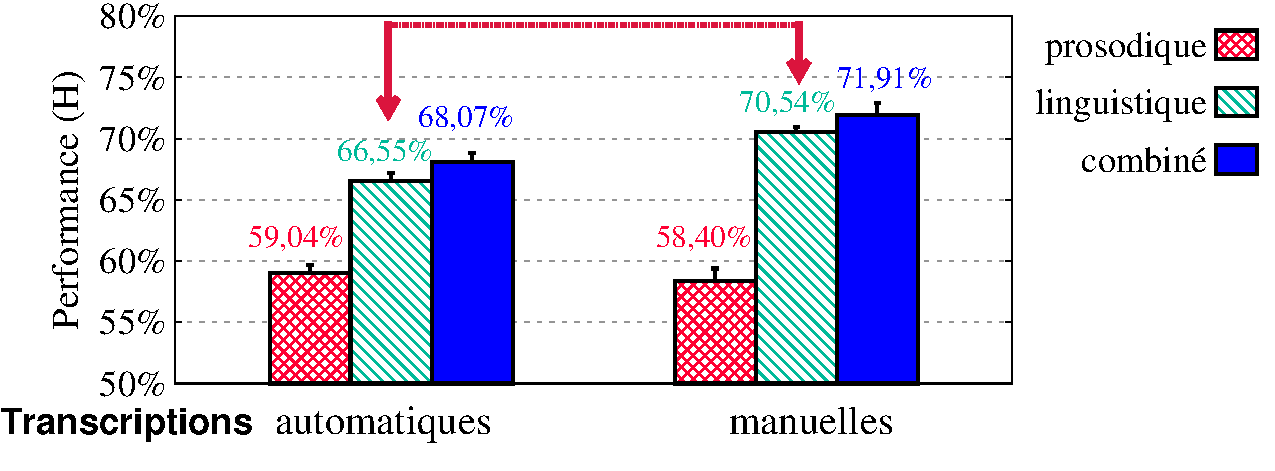
\includegraphics[scale=0.42]{Image/results/JRip_automatic_manual_v3.pdf} \end{center}

\vskip1.1ex
{\scriptsize {\color{purple}$\Rightarrow$} les classifieurs  {\color{ngreen}linguistiques} : perte de performance de 4\% \\ \hskip5ex entre les transcriptions manuelles et automatiques}
}

\only<5-|handout:0>
{
\begin{center} 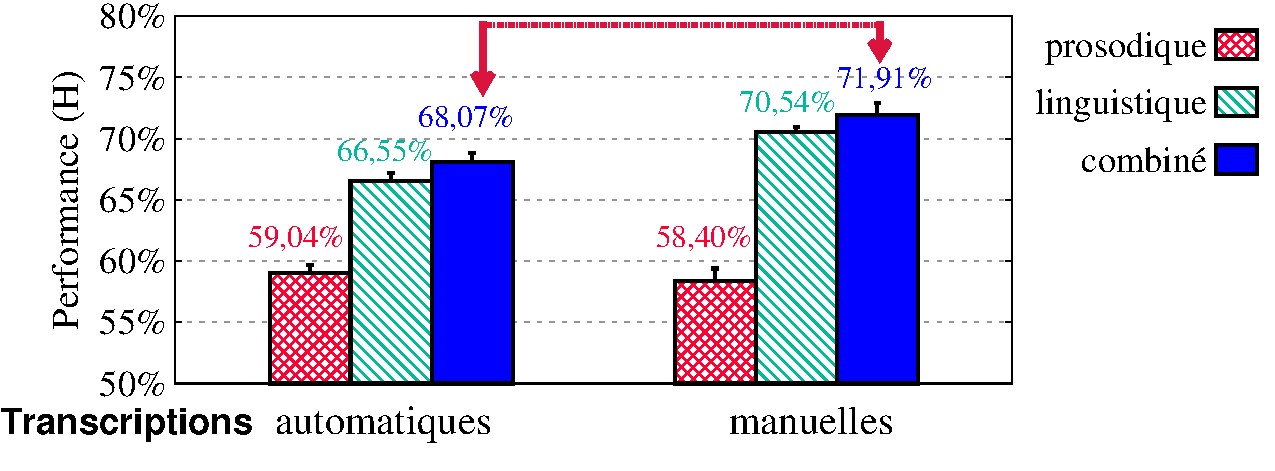
\includegraphics[scale=0.42]{Image/results/JRip_automatic_manual_v4.pdf} \end{center}

\vskip1.1ex
{\scriptsize {\color{purple}$\Rightarrow$} les classifieurs  {\color{blue}combinés} : perte de performance de 3,8\% \\ \hskip5ex  entre les transcriptions manuelles et automatiques}
}


\end{frame}


%==============================================================================================================
\begin{frame}[t]{Impact de la parole spontanée}

\begin{itemize}
\item {\footnotesize Classification sur \textbf{\color{purple}parole préparée} (ESTER2) et \textbf{\color{purple}spontanée} (ETAPE)}
\end{itemize}

\vspace*{-0.1ex}

\begin{center}
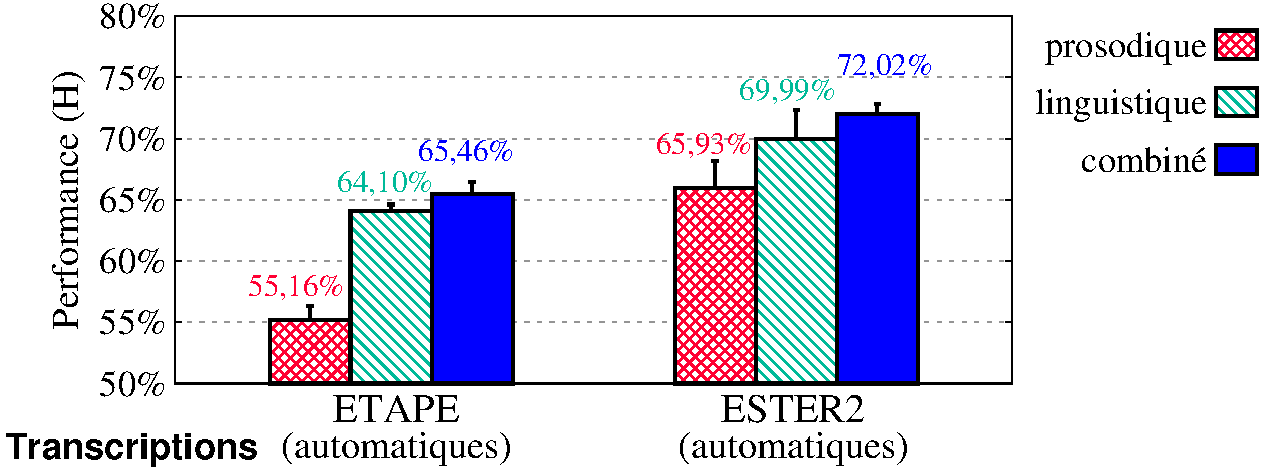
\includegraphics[scale=0.42]{Image/results/JRip_automatic_EsterVsEtape.pdf}
\end{center}

\vskip1.1ex
{\scriptsize {\color{purple}$\Rightarrow$} meilleure performance sur parole préparée (ESTER2) \\\vskip0.5ex\hskip5ex que sur parole spontanée (ETAPE) }


\end{frame}




%==============================================================================================================
\begin{frame}[t]{Impact des frontières des phrases}

\begin{itemize}
\vspace*{-1ex}
\item {\footnotesize Classification sur \textbf{\color{purple}frontières des phrases} imparfaites}

	\begin{itemize}
	\vskip0.1ex
	\item[$\rightarrow$] modifie les frontières prédéfinies des phrases

	{\scriptsize

	\vskip1.5ex\hskip1ex {\color{darkcerulean}$\triangleright$} en décalant chaque frontière (gauche ou droite) au hasard {\color{purple}$\pm300ms$}

	\vskip1ex\hskip1ex {\color{darkcerulean}$\triangleright$} en décalant chaque frontière (gauche ou droite) au hasard {\color{purple}$\pm1000ms$}

	\vskip1ex\hskip1ex {\color{darkcerulean}$\triangleright$} en extrayant le plus long segment délimité par des silences
	}
	\end{itemize}
\end{itemize}


\only<2->
{
\begin{center}
\vskip-0.5ex 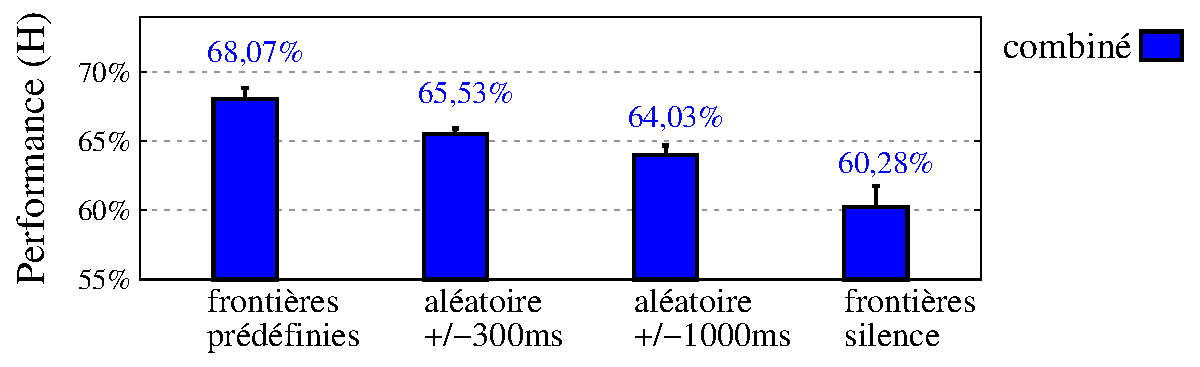
\includegraphics[scale=0.42]{Image/results/differentBoundaries-JRip_onAutomatic_legendPLC.pdf}
\end{center}

{\scriptsize
{\vskip-1.5ex\color{purple}$\Rightarrow$} la perte de performance varie entre 2,5\% et 7,8\%

\vskip1ex {\color{purple}$\Rightarrow$} 65\% d'entrées correctement classées pour des petites variations
}
}

\end{frame}


%==============================================================================================================
\subsection*{Conclusions}
\begin{frame}[t]{Conclusions sur la détection de questions}

\begin{itemize}
{\footnotesize
\vskip2ex
\item la combinaison de paramètres prosodiques et linguistiques offre \\la meilleure performance de classification \\
		\vskip1ex\hskip3ex {\color{darkcerulean}$\rightarrow$} 72\% sur les transcriptions manuelles
		\vskip1ex\hskip3ex {\color{darkcerulean}$\rightarrow$} 68\% sur les transcriptions automatiques

\vskip3ex
\item l'essentiel de l'information pour la détection de la modalité des énoncés provient du contenu linguistique de l'énoncé

\vskip3ex
\item la prosodie apporte un complément d'information

\vskip3ex
\item meilleure performance sur parole préparée que sur parole spontanée

\vskip3ex
\item il est important de bien définir les frontières de phrases pour la tâche de la détection de questions

}
\end{itemize}

\end{frame}



%==============================================================================================================
\section{Conclusions générales}
\begin{frame}[t]{Modèles hybrides}

\begin{itemize}
\vskip3ex
\item Conclusions
	\begin{itemize}
	\vskip1.5ex
	\item combinaison mots et syllabes est une approche prometteuse

	\vskip1ex
	\item permet d'approximer les prononciations de mots hors-vocabulaire
	\end{itemize}

\vskip3ex
\item Perspectives
	\begin{itemize}
	\vskip1.5ex
	\item \textbf{\color{purple}augmenter la quantité des syllabes} dans le corpus d'apprentissage %apprentissage de \textbf{\color{purple} plus grands modèles hybrides}

		\begin{itemize}
		\vskip2ex
		\item[$\Rightarrow$] combiner des données de parole transcrites manuellement \\\vskip0.1ex avec des données purement textuelles

		\vskip1ex
			\vskip1ex\hskip0.1ex {\color{darkcerulean}$\triangleright$} {\scriptsize comment passer du texte \\\hskip5ex à une phonétisation représentative de prononciations}
		\vskip1ex
			\vskip1ex\hskip0.1ex {\color{darkcerulean}$\triangleright$} {\scriptsize comment gérer les e-muets et les liaisons}
		\end{itemize}
	\end{itemize}
\end{itemize}

\end{frame}


%==============================================================================================================
\begin{frame}[t]{Ajout de nouveaux mots}

\begin{itemize}
\vskip3ex
\item Conclusions
	\begin{itemize}
	\vskip1.5ex
	\item notre approche d'utiliser la similarité entre mots pour \\\vskip1ex l'ajout de nouveaux n-grammes dans un modèle est efficace
	\end{itemize}

\vskip3ex
\item Perspectives
	\begin{itemize}
	\vskip2ex
	\item prendre en compte \textbf{\color{purple}plus d'information} pour chercher \\ des mots similaires pour un nouveau mot

	\vskip2ex
	\item \textbf{\color{purple}selectionner les n-grammes} à insérer dans le modèle

	\vskip2ex
	\item \textbf{\color{purple} améliorer les modèles de langage habituels}\hskip-10ex

		\begin{itemize}
		\vskip1ex
		\item[$\rightarrow$] {\scriptsize en estimant de nouveaux n-grammes pour les mots peu fréquents dans le corpus textuel d’apprentissage}
		\end{itemize}
	\end{itemize}
\end{itemize}

\end{frame}



%==============================================================================================================
\begin{frame}[t]{Détection de questions}

\begin{itemize}
\vskip3ex
\item Conclusions
	\begin{itemize}
	\vskip1.5ex
	\item bonne performance de classification: 72\% sur les transcriptions manuelles et 68\% sur les transcriptions automatiques
	\end{itemize}

\vskip3ex
\item Perspectives
	\begin{itemize}
	\vskip2ex
	\item évaluer la performance du système en contexte réel de dialogue

	\vskip2ex
	\item déterminer l'\textbf{\color{purple}impact de fausses détections} sur la compréhension du message transcrit par des personnes sourdes

	\vskip2ex
	\item prendre en compte \textbf{\color{purple}mesures de confiance sur les mots}
\end{itemize}

\end{itemize}


\end{frame}



%==============================================================================================================
\begin{specialframe}

\begin{center}
\textcolor{purple}{\huge \hspace*{-3ex}\textbf{Merci pour votre\\\vskip0.2cm\hspace*{-3ex} attention !}}
\end{center}

\end{specialframe}


%==============================================================================================================
\begin{specialframe}

\begin{center}
\textcolor{purple}{\huge \hspace*{-3ex}\textbf{Questions ?}}
\end{center}

\end{specialframe}



%==============================================================================================================
% Annexes
%==============================================================================================================

%==============================================================================================================
\begin{specialannexe}

\begin{itemize}
\vskip2ex
\item Taux d'erreur phonétique \textbf{\color{purple} PER} (\textit{Phoneme Error Rate})
\end{itemize}

\vskip5ex\hskip5ex
$PER=\frac{{\color{red}\#Insertions}\ +\ {\color{ngreen}\#Omissions}\ +\ {\color{blue}\#Substitutions}}{\text{\textit{\#phonèmes}}}$

\vskip5ex
\hspace{9ex}\begin{beamerboxesrounded}[width=0.4\textwidth,shadow=fasle]{}
	\ttfamily{\footnotesize
	\begin{tabular}{lccccc}
	\textbf{\color{purple} REF:}  & b 				& on 	  & ge &  u 			& \textbf{\color{ngreen}r} \\
	\textbf{\color{purple} HYP:} & \textbf{\color{blue}r} & \textbf{\color{blue}an} & ge & \textbf{\color{blue}swa} & * 		\\ \hline
	%\vspace{-0.3cm}\rule{60mm}{0.7pt}
	\textbf{\color{purple} EVAL:} & \textbf{\color{blue}S} & \textbf{\color{blue}S} & & \textbf{\color{blue}S} & \textbf{\color{ngreen}O} \\
	\end{tabular}
	}
\end{beamerboxesrounded}


\end{specialannexe}


%==============================================================================================================
\begin{specialannexe}

\begin{itemize}

\item 24 paramètres prosodiques calculés sur la phrase entière

	\begin{itemize}
	\vskip2ex
	\item 2 paramètres \textbf{\color{purple}généraux}
		\begin{itemize}
		\item la durée du segment
		\item la vitesse d'élocution
		\end{itemize}

	\vskip2ex
	\item 4 paramètres liés à l'\textbf{\color{purple}énergie}
		\begin{itemize}
		\item la moyenne et l'écart type des log-énergies des voyelles
		\item la pente des logarithmes des énergies
		\item la pente "finale" des logarithmes des énergies
		\end{itemize}

	\vskip2ex
	\item 18 paramètres liés à la \textbf{\color{purple}fréquence fondamentale} (F0)
		\begin{itemize}
		\item le nombre des trames ayant des valeurs F0 ($\ne0$)
		\item la moyenne et l'écart type des valeurs F0 ($\ne0$) des voyelles
		\item la dernière valeur F0 ($\ne0$)
		\item la pente de F0
		\item la pente "finale" de F0
		\item 7 paramètres calculés sur des segments "isolés"
		\item 5 paramètres calculés sur des trames consécutives \\(ignorant les valeurs F0 nulles)
		\end{itemize}

	\end{itemize}

\end{itemize}

\end{specialannexe}



%==============================================================================================================
\begin{specialannexe}

\vskip-1ex
{\scriptsize
\centering
\begin{tabular}{|r|l|}
\hline
id.	& description 									\\ \hline
C0	& la durée du segment (nombre de trames)					\\
C1	& la vitesse d'élocution (nombre de voyelles par seconde) 			\\ \hline
C2,C3	& la moyenne et l'écart type des logarithmes des énergies des voyelles  	\\
C4	& la pente des logarithmes des énergies  					\\
C5	& la pente ``finale" des logarithmes des énergies				\\ \hline
C6	& le nombre des trames ayant des valeurs F0 non-nulles	 			\\
C7,C8	& la moyenne et l'écart type des valeurs F0 (non-nulles) des voyelles 		\\
C9	& la dernière valeur F0 (non nulle)						\\
C10	& la pente de F0 				 				\\
C11	& la pente ``finale" de F0 							\\
C12	& la pente de F0 minimale (sur segment isolé)					\\
C13	& la pente de F0 maximale (sur segment isolé)					\\
C14	& le nombre de pentes de F0 ascendantes (sur segments isolés)  			\\
C15	& le nombre de pentes de F0 descendantes (sur segments isolés)  		\\
C16	& la moyenne des pentes de F0 ascendantes (sur segments isolés) 		\\
C17	& la moyenne des pentes de F0 descendantes (sur segments isolés) 		\\
C18	& la déviation moyenne des pentes de F0 (sur segments isolés) 			\\
C19	& le nombre de pentes de F0 ascendantes (sur trames consécutives)	  	\\
C20	& le nombre de pentes de F0 descendantes (sur trames consécutives)  		\\
C21	& la moyenne des pentes de F0 ascendantes (sur trames consécutives) 		\\
C22	& la moyenne des pentes de F0 descendantes (sur trames consécutives) 		\\
C23	& la déviation moyenne des pentes de F0 (sur trames consécutives) 		\\ \hline
\end{tabular}
}

\end{specialannexe}

%==============================================================================================================
\begin{specialannexe}

\vskip3ex
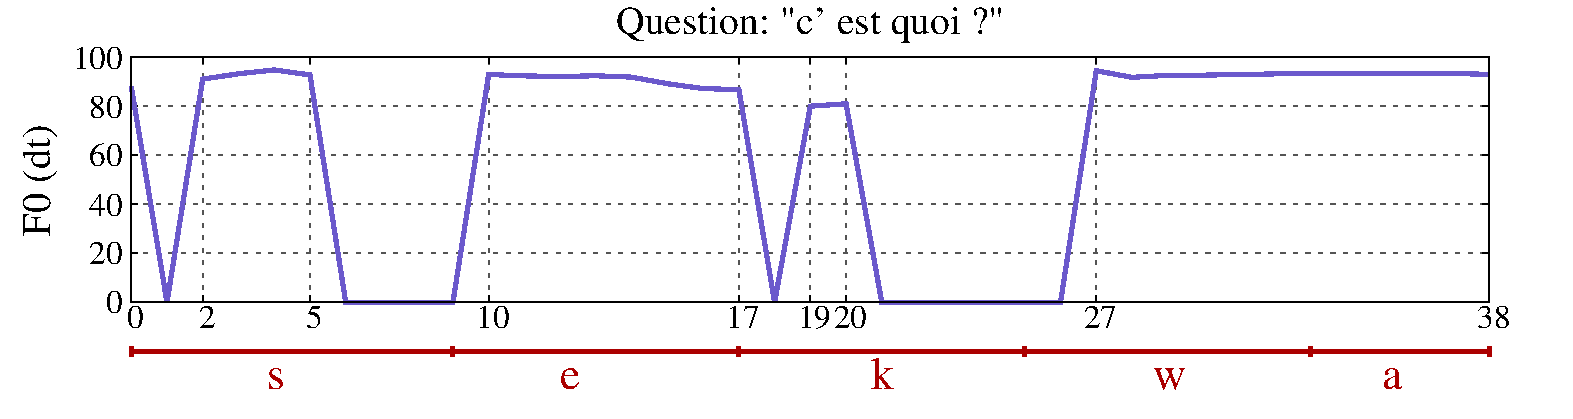
\includegraphics[scale=0.4]{Image/picture/F0prosody.pdf}
\vskip5ex
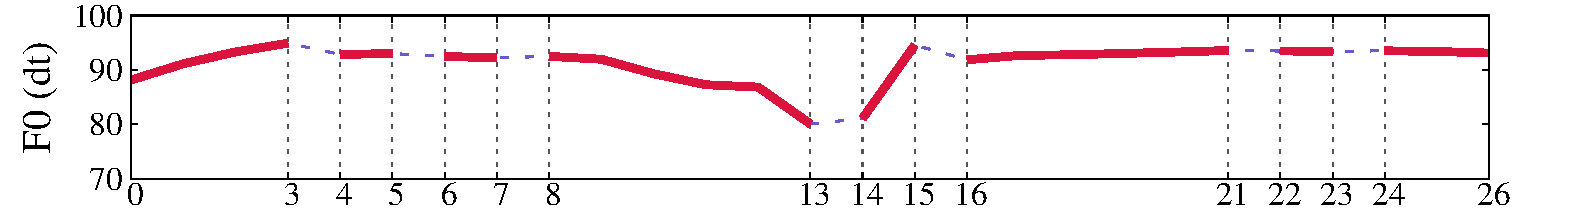
\includegraphics[scale=0.4]{Image/picture/F0prosody_c.pdf}

\end{specialannexe}

%==============================================================================================================
\begin{specialannexe}

\begin{itemize}

\vskip1ex
\item probabilité que la phrase soit une question {\footnotesize (\textbf{\color{blendedblue} lexLLR, synLLR})}
	\vskip1ex\hskip3ex {\footnotesize {\color{darkcerulean}$\rightarrow$} par rapport à deux modèles de langage de référence}
\end{itemize}


\vskip2ex
\begin{columns}
\begin{column}{.05\textwidth}
\end{column}
\begin{column}{.6\textwidth}
\vskip-3ex
\scriptsize
  $$\text{LLR(phrase)}=\text{Log}\left(\frac{\text{P(phrase} \rvert \text{\color{purple}ML-question)}}{\text{P(phrase} \rvert \text{\color{purple}LM-affirmation)}}\right)$$

    \hskip5ex{\color{darkcerulean}$\ast$} LLR $\geq$ 0  $\rightarrow$ susceptible d'être une question \\
    \hskip5ex{\color{darkcerulean}$\ast$} LLR $\textless$ 0 $\rightarrow$ susceptible d'être une affirmation
\end{column}
\begin{column}{.01\textwidth}
\end{column}
\begin{column}{.3\textwidth}
	\hskip-3ex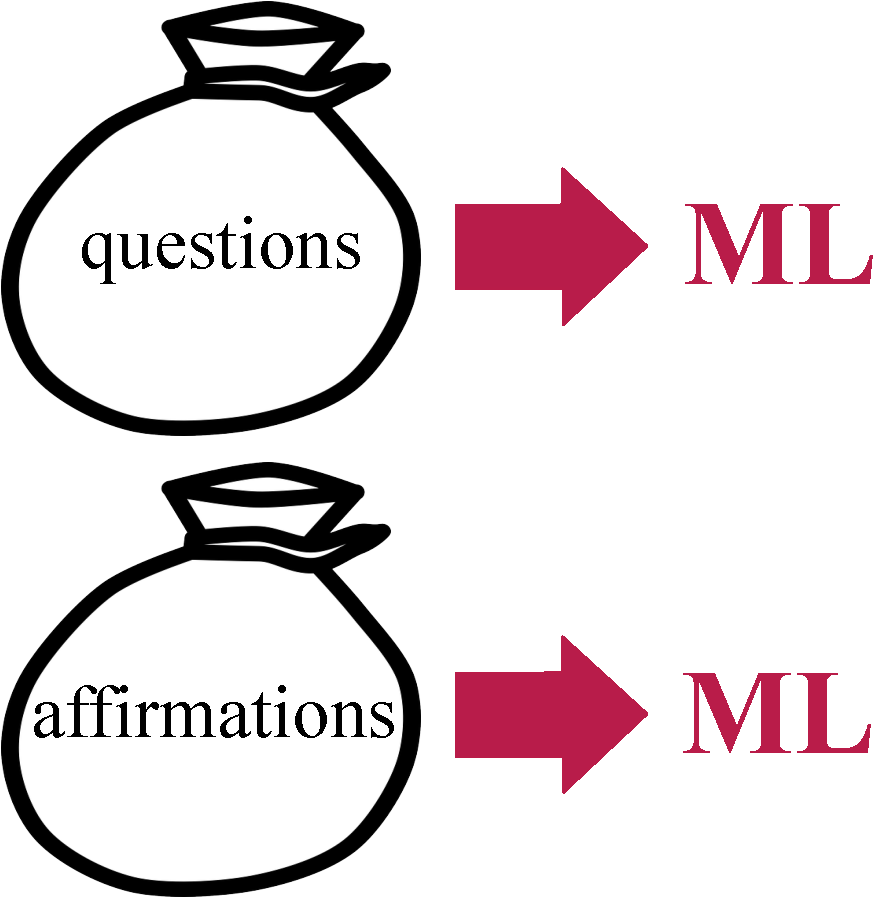
\includegraphics[scale=0.14]{Image/picture/LM-qs-fr.pdf}
\end{column}
\end{columns}

\vskip4ex
\begin{columns}
\begin{column}{0.45\textwidth}
	\begin{beamerboxesrounded}[width=0.9\textwidth,lower=lowcol,shadow=false]{}
	\centering
	\scriptsize
	  \textbf{\color{purple}lexLLR} \\
  	  \vskip-1ex{\color{darkcerulean}\rule{40mm}{0.5pt}}\\
	  modèles de langage \textbf{\color{purple}lexicaux} \\
	  appliqués sur la \textbf{\color{purple}séquence de mots}
	\end{beamerboxesrounded}
\end{column}
\begin{column}{0.55\textwidth}
	\begin{beamerboxesrounded}[width=0.8\textwidth,lower=lowcol,shadow=false]{}
	\centering
	\scriptsize
	  \textbf{\color{purple}synLLR} \\
  	  \vskip-1ex{\color{darkcerulean}\rule{40mm}{0.5pt}}\\
  	   modèles de langage  \textbf{\color{purple}syntaxique} appliqués \\
	   \hskip1.5ex sur la  \textbf{\color{purple}séquence de classes grammaticales}
	\end{beamerboxesrounded}
\end{column}
\end{columns}

\end{specialannexe}

%=====================================================================================================================
\begin{specialannexe}

{\footnotesize Corpus textuel GigaWord}
	\vskip0.4ex\hskip3ex{\color{darkcerulean}$\ast$} {\scriptsize extraction d'\textbf{\color{blendedblue}affirmations} : phrases se finissant par un '.' [\#16M]}
	\vskip0.1ex\hskip3ex{\color{darkcerulean}$\ast$} {\scriptsize extraction de \textbf{\color{blendedblue}questions} :  phrases se finissant par un '?' [\#89K]}


\vskip2ex
\begin{beamerboxesrounded}[width=0.8\textwidth,shadow=false]{\footnotesize séquences de mots}
	{\scriptsize
	\begin{tabular}{r|l}
	question	& à quel moment le raid a décidé d'intervenir?		\\ \hline
	affirmation	& nous sommes ensemble pour 60 minutes.			\\
	\end{tabular}
	}
\end{beamerboxesrounded}

\begin{center}
	\vskip-3ex
	$\Downarrow$

	\vskip-0.5ex
	{\scriptsize les \textbf{\color{purple}modèles de langage lexicaux} des questions et des affirmations}
\end{center}

\vskip1ex
\begin{beamerboxesrounded}[width=0.8\textwidth,shadow=false]{\footnotesize séquences de classes grammaticales (POS) }
{\scriptsize
	\begin{tabular}{r|l}
	{\scriptsize question} 	&
	    {\tiny PRP PRO$\mathalpha{:\,}$REL NOM DET$\mathalpha{:\,}$ART NOM VER$\mathalpha{:\,}$pres VER$\mathalpha{:\,}$pper PRP VER$\mathalpha{:\,}$infi }  \\ \hline
	{\scriptsize affirmation} &
	    {\tiny  PRO$\mathalpha{:\,}$PER VER$\mathalpha{:\,}$pres ADV PRP NUM NOM}					\\
	\end{tabular}
}
\end{beamerboxesrounded}

\begin{center}
	\vskip-3ex
	$\Downarrow$

	\vskip-0.5ex
	{\scriptsize les \textbf{\color{purple}modèles de langage syntaxiques} des questions et des affirmations}
\end{center}

\end{specialannexe}


%=====================================================================================================================
\begin{specialannexe}


{\scriptsize \textbf{Exemple d'une fonction JRip}}

\bigskip

%(LogP <= -0.567956) and (LogT >= -0.103107) and (LogT <= 0.029789)   			=> class=0.00 (1832.0/200.0)
%(LogP >= -1.30874)  and (LogP <= -0.294368) and (LogT <= 0.011847) 			=> class=0.00 (1587.0/272.0)
%(LogP >= -1.524116) and (LogP <= -0.190467) and (LogT <= 0.122767) and (iF <= 0) 	=> class=0.00 (2833.0/699.0)
%(LogP >= -0.1869)   and (LogP <= 0.154082)  and (LogT <= 0.046103) and (iF <= 0) 	=> class=0.00 (2280.0/729.0)
%(LogP >= -1.052433) and (LogP <= -0.007292) and (iF <= 0) 				=> class=0.00 (2321.0/945.0)
%(LogP <= 0.64342)   and (LogT >= -0.087156) and (LogT <= 0.0275) and (iF <= 0) 	=> class=0.00 (730.0/321.0)
% => class=1.00 (9227.0/1988.0)

{\tiny
\hskip-9.5ex
\renewcommand{\arraystretch}{1.8}
\begin{tabular}{lllllll|l}
(LogP $\leq$ -0.567956) & \& & (LogT $\geq$ -0.103107) & \& & (LogT $\leq$ 0.029789) 	& &			& $\Rightarrow$ class=Affirmation \\
(LogP $\geq$ -1.30874)  & \& & (LogP $\leq$ -0.294368) & \& & (LogT $\leq$ 0.011847) 	& &			& $\Rightarrow$ class=Affirmation \\
(LogP $\geq$ -1.524116) & \& & (LogP $\leq$ -0.190467) & \& & (LogT $\leq$ 0.122767) 	& \& & (iF $\leq$ 0)	& $\Rightarrow$ class=Affirmation \\
(LogP $\geq$ -0.1869)   & \& & (LogP $\leq$ 0.154082)  & \& & (LogT $\leq$ 0.046103) 	& \& & (iF $\leq$ 0)	& $\Rightarrow$ class=Affirmation \\
(LogP $\geq$ -1.052433) & \& & (LogP $\leq$ -0.007292) & \& & (iF $\leq$ 0) 		& &			& $\Rightarrow$ class=Affirmation \\
(LogP $\leq$ 0.64342)   & \& & (LogT $\geq$ -0.087156) & \& & (LogT $\leq$ 0.0275)	& \& & (iF $\leq$ 0)  	& $\Rightarrow$ class=Affirmation \\\hline
else & & & & & & &  $\Rightarrow$ class=Question
\end{tabular}
}

\bigskip

{\scriptsize

Nombre de règles : 7

\smallskip
\textbf{\color{purple} Performance 66,95\%} (questionsCC=64,57\%, affirmationsCC=69,51\%)
}


\end{specialannexe}




%==============================================================================================================
\begin{specialannexe}

Matrice de confusion entre questions et affirmations

\vskip1ex
{\scriptsize
\hskip-0.1ex
\begin{tabular}{|p{1.7cm}|p{1cm}|p{1.6cm}|p{1.6cm}|p{2cm}}
\cline{2-4}
\multicolumn{1}{c|}{}	& \multirow{2}{*}{nombre} 	& classé 		& classé 		& \multicolumn{1}{c}{}		\\
\multicolumn{1}{c|}{}	&  				& question		& affirmation 		& \multicolumn{1}{c}{}		\\ \cline{1-4}
question   		&  940 				& \textbf{631} 		& 309    		& \textbf{questionsCC=67,13\%} 	\\ \cline{1-4}
affirmation  		& 7708 				& 2136 			& \textbf{5572}  	& \textbf{affirmationsCC=72,39\%} \\ \cline{1-4}
\multicolumn{4}{c}{}											& \vskip-1.5ex \textbf{\color{purple}H=69,61\%}	\\
\end{tabular}
}

{\footnotesize
\begin{itemize}
\vskip2ex
\item \textbf{\color{purple}Précision et rappel sur questions}

	\vskip1ex
	\begin{columns}
	\begin{column}{0.15\textwidth}
	\end{column}
	\begin{column}{0.43\textwidth}
		\renewcommand{\arraystretch}{1.3}
		\begin{tabular}{rll}
		${\color{blendedblue}\text{précisionQ}}=$ 	& \hskip-2.1ex $\frac{631}{631+2136}=$ 	& \hskip-2ex ${\color{blendedblue}22,80\%}$ \\
		${\color{blendedblue}\text{rappelQ}}=$ 		& \hskip-2ex $\frac{631}{631+309}=$ 	& \hskip-2ex ${\color{blendedblue}67,13\%}$ \\
		\end{tabular}
	\end{column}
	\begin{column}{0.42\textwidth}
		$\Rightarrow {\color{blendedblue}\text{fmesureQ}} = {\color{blendedblue}34,09\%}$
	\end{column}
	\end{columns}

\vskip2ex
\item \textbf{\color{purple}Précision et rappel sur affirmations}

	\vskip1ex
	\begin{columns}
	\begin{column}{0.15\textwidth}
	\end{column}
	\begin{column}{0.43\textwidth}
		\renewcommand{\arraystretch}{1.3}
		\begin{tabular}{rll}
		${\color{blendedblue}\text{précisionA}}=$	& \hskip-2ex $\frac{5572}{5572+309}=$	& \hskip-2ex ${\color{blendedblue}94,75\%}$ \\
		${\color{blendedblue}\text{rappelA}}=$ 		& \hskip-2ex $\frac{5572}{5572+2136}=$ 	& \hskip-2ex ${\color{blendedblue}72,29\%}$ \\
		\end{tabular}
	\end{column}
	\begin{column}{0.42\textwidth}
		$\Rightarrow {\color{blendedblue}\text{fmeasureA}} = {\color{blendedblue}82,01\%}$
	\end{column}
	\end{columns}

\vskip2ex
\item \textbf{\color{purple}moyenne pondérée de la F-mesure} = {\color{blendedblue}76,80\%}

\end{itemize}
}

\end{specialannexe}



%==============================================================================================================
\begin{specialannexe}

Performance d'un système qui répond au hasard (50\%-50\%)

\vskip1ex
{\scriptsize
\hskip-0.1ex
\begin{tabular}{|p{1.7cm}|p{1cm}|p{1.6cm}|p{1.6cm}|p{2cm}}
\cline{2-4}
\multicolumn{1}{c|}{}	& \multirow{2}{*}{nombre} 	& classé 		& classé 		& \multicolumn{1}{c}{}			\\
\multicolumn{1}{c|}{}	&  				& question		& affirmation 		& \multicolumn{1}{c}{}			\\ \cline{1-4}
question   		&  940 				& \textbf{470} 		& 470    		& \textbf{questionsCC=50,00\%} 		\\ \cline{1-4}
affirmation  		& 7708 				& 3854 			& \textbf{3854}  	& \textbf{affirmationsCC=50,00\%} 	\\ \cline{1-4}
\multicolumn{4}{c}{}											& \vskip-1.5ex \textbf{\color{purple}H=50,00\%}	\\
\end{tabular}
}

{\footnotesize
\begin{itemize}
\vskip2ex
\item \textbf{\color{purple}Précision et rappel sur questions}

	\vskip1ex
	\begin{columns}
	\begin{column}{0.15\textwidth}
	\end{column}
	\begin{column}{0.43\textwidth}
		\renewcommand{\arraystretch}{1.3}
		\begin{tabular}{rll}
		${\color{blendedblue}\text{précisionQ}}=$ 	& \hskip-2.1ex $\frac{470}{470+3854}=$ 	& \hskip-2ex ${\color{blendedblue}10,87\%}$ \\
		${\color{blendedblue}\text{rappelQ}}=$ 		& \hskip-2ex $\frac{470}{470+470}=$ 	& \hskip-2ex ${\color{blendedblue}50,00\%}$ \\
		\end{tabular}
	\end{column}
	\begin{column}{0.42\textwidth}
		$\Rightarrow {\color{blendedblue}\text{fmesureQ}} = {\color{blendedblue}17,86\%}$
	\end{column}
	\end{columns}


\end{itemize}
}

\end{specialannexe}


%=====================================================================================================================
\begin{specialannexe}

\vskip-1ex
\textbf{Add new words into a language model}
\vskip-2ex
\rule{105mm}{0.7pt}

{\scriptsize
\begin{tabular}{l}
{\color{blue}newLM} $\leftarrow$ LM			\\
{\color{blue}newNgrams} $\leftarrow$ $\varnothing$	\\
\emph{\color{darkgray}\# process the reference ngrams}	\\
{\textbf{for each} ngram $\in$ LM}			\\
	\hspace*{5ex} {\textbf{for each} kW $\in$ similarWords(\textbf{\color{red}nW})}		\\
		\hspace*{10ex} \textbf{if} {$contains$(ngram, kW)} \textbf{then}		\\
			\hspace*{15ex} ngram\textbf{'} $\leftarrow$ $replace$(ngram, kW, nW)	\\
			\hspace*{15ex} push({\color{blue}newNgrams}, ngram\textbf{'})		\\
		\hspace*{10ex} \textbf{end if}							\\
	\hspace*{5ex} \textbf{end for}								\\
\textbf{end for} \\
\emph{\color{darkgray}\# choose the new ngrams to add to the newLM}	\\
S  $\leftarrow$ $getUniqueSequences$({\color{blue}newNgrams})		\\
{\textbf{for each} seq $\in$ S}						\\
	\hspace*{5ex} \textbf{if} {$frequency$(seq) = 1} \textbf{then} 	\\
		\hspace*{10ex} prob  $\leftarrow$ $getProbability$(seq)	\\
	\hspace*{5ex} \textbf{else} 					\\
		\hspace*{10ex} P  $\leftarrow$ $getProbabilities$(seq)	\\
		\hspace*{10ex} prob $\leftarrow$ $medianProbability$(P)	\\
	\hspace*{5ex} \textbf{end if} 					\\
	\hspace*{5ex} push({\color{blue}newLM},  ``prob seq'')			\\
\textbf{end for} \\
\end{tabular}
}

\end{specialannexe}





\end{document}


